% \section{Vorgehen und Methodik}

%#############################
% Forschungsstand zur künstlichen Intelligenz
%#############################
\cleardoublepage
\section{Künstliche Intelligenz: Grundlagen und Ansätze in der Praxis}
\label{chap:ai}

\todo[inline, color=orange]{Eine Einleitung zur Definition von künstlicher Intelligenz geben. Auf den Begriff Machine Learning eingehen}

% \todo[inline, color=igloo]{Vorschlag: Hier könntest Du mit dem Begriff KI beginnen und die Problematik ansprechen, dass zwar viele davon sprechen, aber (falls überhaupt) nur wenige wissen, was darunter zu verstehen ist. Vieles, was heute angeboten wird, basiert auf ML-Ansätzen, wie z.B. und dann kannst Du best practices aufweisen.}

Die künstliche Intelligenz ist ein in der Literatur oft diskutiertes Themengebiet. Bereits 2009 geben \textcite{Russell2009} auf über 1000 Seiten einen noch immer aktuellen und sehr umfangreichen Überblick über dieses Themengebiet. Weiter vertiefen die beiden Autoren viele Teilgebiete der künstlichen Intelligenz und erläutern grundlegende Konzepte ausführlich.

% Einen etwas mathematischeren Überblick über das Thema künstliche Intelligenz geben \textcite{Goodfellow2016}. Die Diskussion reicht von den absoluten Grundlagen, der linearen Algebra, bis hin zu Deep Generative Models, eine fortgeschrittene Anwendung der künstlichen Intelligenz~\autocite{Goodfellow2016}.

Es kann gesagt werden, dass in der Grundlagenforschung zur künstlichen Intelligenz bereits viele Forschungsergebnisse vorliegen. Es werden etliche, etablierte und experimentelle, Techniken diskutiert und täglich weiterentwickelt. Zur Automatisierung eines Geschäftsprozesses und somit für die Entwicklung eines Prototypen für die AXA Gesundheitsvorsorge stehen unzählige Möglichkeiten zur Verfügung.

Dieses Kapitel gibt ein Überblick über das Themengebiet der künstlichen Intelligenz. Es werden für diese Arbeit relevante Techniken, Konzepte und Begriffe erläutert. Es werden Konzepte und Metriken vorgestellt, welche verwendet werden, um eine künstliche Intelligenz zu bewerten. Zum Schluss wird aufgezeigt, wie eine künstliche Intelligenz modelliert und die finale Architektur entsteht.

\subsection{Natural Language Processing}

Natural Language Processing (kurz NLP) beschreibt das Gebiet der Forschung und Anwendung von Computern um natürliche Sprache, in Wort und Schrift, zu verstehen und verarbeiten. NLP umfasst diverse Forschungsfelder wie beispielsweise die maschinelle Übersetzung, die Spracherkennung sowie die Informationsextraktion~\autocite{Chowdhury2003}. 

Für diese Arbeit ist das Themengebiet des Natural Language Processing insofern relevant, als dass es die Grundlage für die Verarbeitung von Rechnungen bildet. Mit Techniken aus diesem Gebiet werden die Inhalte der Rechnungen vom Computer verstanden und verarbeitet.

\subsection{Neuronale Netzwerke}
\label{chap:neuron}

Abgesehen von Rechenaufgaben sind Menschen Leistungsfähiger als Computer. Wir sind beispielsweise in der Lage, Gesichter zu erkennen oder in einem dunklen Raum Personen anhand Ihrer Stimme zu identifizieren. Der interessanteste Unterschied des menschlichen Gehirns zu einem Computer ist der Fakt, dass unser Gehirn lernt, ohne eine Softwareaktualisierung zu erhalten. Wir brauchen nicht erst eine neue Software, um das Fahrradfahren zu erlernen~\autocite{Krogh2008}. Doch wie funktioniert das?

Die Berechnungen des menschlichen Gehirn werden durch hoch vernetzte Neuronen gemacht. Dabei interagieren die Neuronen mit Stromimpulsen durch die neuronale Verkabelung, bestehend aus Nervensäulen, Synapsen und Zellfortsätzen. 1943 modellierten McCulloch und Pitts Neuronen als Schalter, welche aufgrund der eingehenden Signale ein- oder ausgeschaltet werden. Die Gewichtung der eingehenden Signale waren dabei die Synapsen. Aus diesem Modell entstand das Konzept von neuronalen Netzwerken\todo{Search \& Replace, überall gleich schreiben}~\autocite{Krogh2008}.

Ein Neuron wird dabei als eine Threshold Unit (vgl. Abbildung \ref{krogh:a}) modelliert, welche Eingabewerte anderer Units oder externer Quellen erhält. Diese Eingabewerte werden gewichtet und summiert. Liegt die Summe der gewichtet Eingabewerte nun über dem definierten Threshold, so aktiviert sich die Threshold Unit und der Ausgabewert ist 1. Liegt der Wert unter dem Threshold, so ist der Ausgabewert 0.

%\begin{wrapfigure}{l}{0.4\textwidth} 
\begin{figure}[H]
    \captionsetup{width=.9\linewidth}
    \caption[Modell eines Neurons nach McCulloch und Pitts]{Modell eines Neurons nach McCulloch und Pitts. Die sogenannte Threshold Unit erhält $N$ Eingangssignale $x_1, ..., x_N$. Diese Eingangssignale werden mit dem zugehörigen Gewicht $w_1, ..., w_N$ multipliziert und schlussendlich summiert. Die Summe der Gewichte ist 1 $\sum_{i=1}^{N} w_i = 1$, dadurch liegt die Summe der gewichteten Eingangssignale $\sum_{i=1}^{N} w_i x_i = 1$ zwischen $0$ und $1$. Das Modell zeigt nun zwei verschiedene Arten, wie der Ausgabewert eines Neurons modelliert werden kann. Zum einen kann das Modell je nach Erreichung eines Gewissen Threshold ($t$) mit $0$ oder $1$ aktiviert werden. Andererseits kann ein kontinuierlicher Sigmoid (rote Linie) verwendet werden, um einen kontinuierlichen Ausgabewert zwischen $0$ und $1$ zu ermitteln.}
    \label{krogh:a}
    \centering
    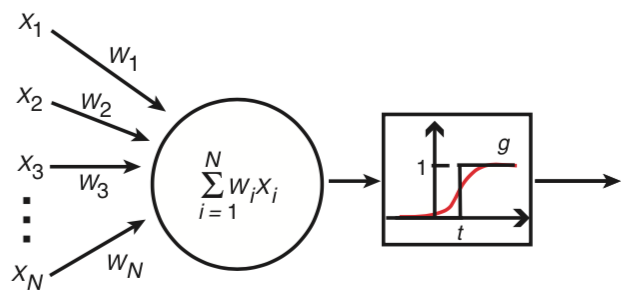
\includegraphics[width=0.5\linewidth]{graphics/krogh/krogh_neural-network.png}
    \caption*{Quelle: \textcite{Krogh2008}}
%\end{wrapfigure}
\end{figure}

Damit ein neuronales Netzwerk leistungsfähig werden kann, muss es ähnlich wie ein Mensch, erst lernen. Für das neuronale Netzwerk bedeutet Lernen, für die Gewichte und den Threshold geeignete Werte zu finden. Dieses computersimulierte Lernen, auch Machine Learning genannt, funktioniert dabei so, dass für die Gewichte der Verbindungen, sprich die Stärke der Synapsen, ein zufälliger Wert gewählt wird. Anschliessend wird eine Übungsaufgabe vom Netzwerk gelöst. Das Resultat des Netzwerks ist zu Beginn höchstwahrscheinlich falsch und die Gewichte im Netzwerk werden mit einem kleinen Schritt angepasst. Es werden dann immer weitere Aufgaben gelöst und die Gewichte entsprechend angepasst bis das Netzwerk die gewünschten Resultate liefert~\autocite{Krogh2008}.
Dieses Training kann durch verschiedene Algorithmen implementiert werden. Einer davon wird im Kapitel \ref{chap:backpropagation} beschrieben.

Seit mehreren Jahren liefern neuronale Netzwerke bessere Resultate als klassische Techniken. Dabei werden neuronale Netzwerk vorwiegend für visuelle Aufgaben und immer häufiger auch zur Verarbeitung Natürlicher Sprache verwendet~\autocite{Olah2014b}.

% \todo[inline]{Say a word on overfitting}

% \todo[inline]{Say something about learning strategies (supervised / unsupervised)}

\subsection{Tiefe neuronale Netzwerke}
\label{chap:deep-neural-nets}

Neuronale Netzwerke finden oft bei Klassifizierungsproblemen Anwendung. Dabei soll aufgrund bestimmter Eingabewerte eine Klasse bestimmt werden. Ein Beispiel dafür ist die Klassifizierung eines Säugetiers in die Klasse Hund oder Katze aufgrund ihrer Merkmale~\autocite{Krogh2008}.

Einfache Netzwerke von Threshold Units können Klassifizierungsprobleme dann Lösen, wenn die Klassen linear separierbar sind. Die Abbildung \ref{krogh:b} veranschaulicht die lineare Separierung mit Hilfe einer Ebene in einem dreidimensionalen Raum. Die Ebene separiert die grünen und roten Punkte voneinander~\autocite{Krogh2008}.

%\begin{wrapfigure}{l}{0.4\textwidth} 
\begin{figure}[H]
    \captionsetup{width=.9\linewidth}
    \caption[Konzept der linearen Separierbarkeit]{Konzept der linearen Separierbarkeit. Die grünen und roten Kreuze liegen, im Gegensatz zu den Punkten, auf der falschen Seite der Ebene. Die Problemstellung ist somit nicht linear separierbar.}
    \label{krogh:b}
    \centering
    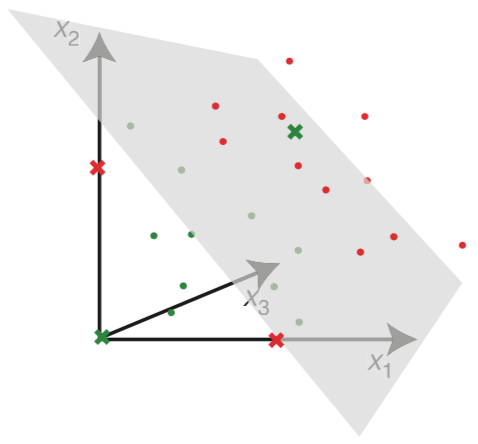
\includegraphics[width=0.4\linewidth]{graphics/krogh/krogh_plane.png}
    \caption*{Quelle: \textcite{Krogh2008}}
%\end{wrapfigure}
\end{figure}

Der Abbildung \ref{krogh:b} ist zu entnehmen, dass die Problemstellung im abgebildeten Fall, wie die meisten Klassifizierungsprobleme, nicht linear separierbar ist. Die roten und grünen Kreuze markieren dabei Punkte, welche auf der falschen Seite der Ebene liegen. Eine Klassifizierung durch ein einfaches Netzwerk von Threshold Units würde die Klasse dieser Datensätze falsch vorhersagen~\autocite{Krogh2008}.

Um das Modell zur Klassifizierung zu verbessern, können weitere Ebenen in den dreidimensionalen Raum eingesetzt werden. Durch eine weitere Ebene ist es dem Modell möglich, mehr Datensätze richtig zu klassifizieren. Neue Ebenen werden mit neuen Schichten von Threshold Units modelliert (vgl. Abbildung \ref{krogh:c}). Diese neuen Schichten, welche zwischen die Eingabe und Ausgabe Schichten platziert werden, werden versteckte Schichten (Hidden Layers) genannt. Ein Modell mit mindestens einer solcher versteckter Schicht wird als tiefes neuronales Netzwerk (Deep Neural Network) bezeichnet~\autocite{Krogh2008}.

% \begin{wrapfigure}{l}{0.4\textwidth} 
\begin{figure}[H]
    \captionsetup{width=.9\linewidth}
    \caption[Modell eines tiefen neuronalen Netzwerks]{Modell eines tiefen neuronalen Netzwerks mit einer versteckten Schicht (Hidden Layer).}
    \label{krogh:c}
    \centering
    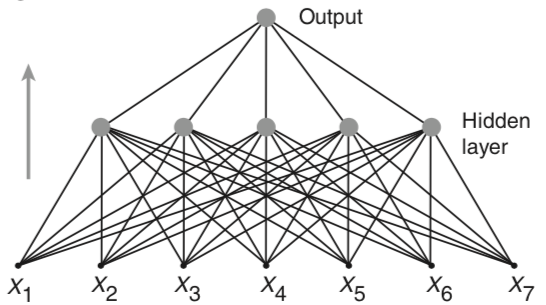
\includegraphics[width=0.4\linewidth]{graphics/krogh/krogh_deep-network.png}
    \caption*{Quelle: \textcite{Krogh2008}}
%\end{wrapfigure}
\end{figure}

Mit immer mehr verfügbarer Rechenkapazität und immer mehr Daten steigt die Popularität tiefer neuronaler Netzwerke gegenüber traditionellen Lernalgorithmen wie der logistischen Regression. Je tiefer und breiter ein neuronales Netzwerk ist und je mehr Trainingsdaten zur Verfügung stehen, desto besser wird es eine Problemstellung lösen können (vgl. Abbildung \ref{scale-drives-ml-progress})~\autocite{MLYearning}.

% \begin{wrapfigure}{l}{0.4\textwidth} 
\begin{figure}[H]
    \captionsetup{width=.9\linewidth}
    \caption{Verhältnis der verfügbaren Daten und der Genauigkeit unterschiedlich grosser neuronaler Netze.}
    \label{scale-drives-ml-progress}
    \centering
    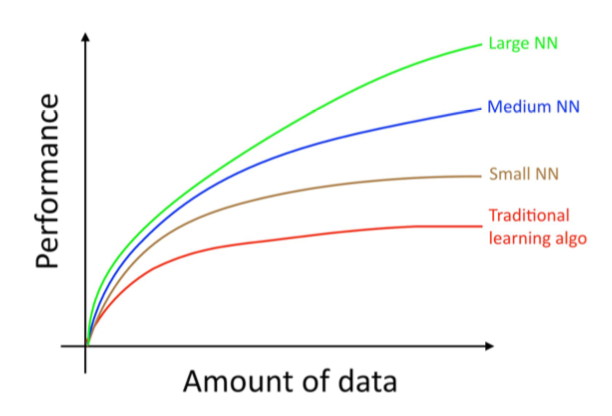
\includegraphics[width=0.4\linewidth]{graphics/scale-drives-ml-progress.png}
    \caption*{Quelle: \textcite{MLYearning}}
%\end{wrapfigure}
\end{figure}

Ein tiefes neuronales Netzwerk stellt aber neue Anforderungen an das Training. Ein Netzwerk mit versteckten Schichten kann nicht mehr auf eine analytische Weise trainiert werden. Aus diesem Grund wird ein komplexerer Lernalgorithmus benötigt. Ein solcher Algorithmus wird im nächsten Kapitel erläutert~\autocite{Krogh2008}. 

Auch ist ein tiefes neuronales Netzwerk anfälliger auswendig zu lernen und birgt somit die Gefahr schlecht zu generalisieren. Dieses sogenannte Overfittig wird im Kapitel \ref{chap:overfitting} erläutert.

\subsection{Backpropagation}
\label{chap:backpropagation}

Da, wie bereits im vorherigen Kapitel erwähnt, tiefe neuronale Netzwerke zu Komplex sind, um mit einem analytischen Ansatz trainiert zu werden, muss ein anderes Vorgehen gefunden werden. Das am meisten angewendete Vorgehen zum Training von tiefen neuronalen Netzwerken ist die sogenannte Backpropagation. Bei der Backpropagation werden erst zufällige Gewichte und Thresholds festgesetzt. Das Netzwerk löst mit diesen zufälligen Gewichten und Thresholds eine erste Übungsaufgabe. Die Abweichung vom erwarteten Resultat (der sogenannte Fehler) wird anschliessend quadriert. Ziel des Backpropagation ist es, diesen quadrierten Fehler zu minimieren. Dies wird erzielt, indem das Verfahren des steilsten Abstiegs, auch Gradientverfahren (englisch gradient descent), angewendet wird. Mit Hilfe dieses Verfahrens, zur Lösung allgemeiner Optimierungsprobleme aus der Numerik, werden nun die Gewichte und der Threshold so angepasst, dass der quadrierte Fehler minimiert werden kann. Dieses Vorgehen wird mit weiteren Übungsaufgaben wiederholt, bis sich der quadrierte Fehler nicht mehr verändert~\autocite{Krogh2008}.

Beim Backpropagation müssen einige Probleme beachtet werden. So kann durch das Gradientverfahren nur ein lokales Minimum gefunden werden. Ob dieses lokale Minimum dem globalen Minimum entspricht, ist nicht bekannt. Das Ergebnis des Trainings ist damit von den zufällig gewählten Startwerten der Gewichte und Thresholds abhängig~\autocite{Krogh2008}.

Die grösste Problematik beim Trainieren von neuronalen Netzwerken, besonders von tiefen neuronalen Netzwerken, ist die Gefahr des sogenannten Overfitting oder Auswendiglernens~\autocite{Krogh2008}.

\subsection{Over- und Underfitting}
\label{chap:overfitting}

Eine Herausforderung der künstlichen Intelligenz beziehungsweise des Machine Learning ist es, auf zuvor unbekannten Daten gute Ergebnisse zu erzielen. Diese Fähigkeit wird als Generalisierung bezeichnet~\autocite{Goodfellow2016}.

Um eine Generalisierung sicherzustellen, wird ein Modell immer auf einem Trainingsdatensatz trainiert und auf einem Testdatensatz validiert. Ziel eines Modells ist es, die Fehler während dem Training (auch Bias genannt) zu minimieren und den Unterschied zwischen der Fehlerquote während dem Training und während der Validierung (auch Varianz genannt) möglichst klein zu halten. Die Nichterreichung dieser Ziele wird Over- respektive Underfitting genannt~\autocite{Goodfellow2016}.

Die Problematik des Underfitting wurde bereits bei der Einführung von tiefen neuronalen Netzwerken, im Kapitel \ref{chap:deep-neural-nets}, angeschnitten. Ein Modell, welches zu wenige Parameter hat, ist nicht in der Lage eine komplexe Problemstellung abzubilden. Das Modell hat somit einen hohes Bias (hohe Fehlerquote auf dem Trainingsdatensatz). In diesem Fall ist es wichtig, das Modell anzupassen. Eine Erhöhung der Anzahl Trainingsdatensätze hilft nicht, den Bias zu reduzieren~\autocite{MLYearning}.

Das sogenannte Overfitting, oder auch Auswendiglernen, bezeichnet die Problematik, dass sich ein Modell aufgrund zu vieler Parameter bei zu wenig Trainingsdaten zu stark an diese Trainingsdaten anpasst. Das Modell kann die Trainingsdaten mit annähernd 100\% Treffergenauigkeit Beurteilen, hat also ein kleines Bias. Soll das Modell dann aber einen neuen Datensatz beurteilen, so sinkt die Treffergenauigkeit erheblich. Das Modell hat eine hohe Varianz und ist nicht in der Lage das gelernte zu generalisieren~\autocite{MLYearning, Krogh2008}.

Die Problematik des Overfitting ist aus der Mathematik bekannt. Hat eine Funktion zu viele freie Parameter, so passt sie sich zu stark an die vorgegebenen Punkte an. Die Abbildung \ref{krogh:d} veranschaulicht diese Problematik anhand von Graphen von Funktionen, welche 8 Punkte fitten sollen. Der grüne Graph ist ein Beispiel des Underfitting. Er hat zu wenige Parameter, um eine tiefe Abweichung zu erreichen. Der pinke Graph zeigt ein Beispiel eines Overfitting. Mit vielen Parametern vermag der Graph alle Punkte perfekt zu schneiden. Die vielen extremen Wendepunkte deuten aber darauf hin, dass der Graph neue Punkte mit hoher Wahrscheinlichkeit nicht schneiden würde. Der blaue Graph gilt als Beispiel für ein gutes Fitting. Der Graph ist nahe an den Punkten, ohne dabei extreme Wendepunkte haben zu müssen~\autocite{Krogh2008}.

% \begin{wrapfigure}{l}{0.4\textwidth} 
\begin{figure}[H]
    \captionsetup{width=.9\linewidth}
    \caption{Over- und Underfitting dargestellt anhand von Graphen von Funktionen}
    \label{krogh:d}
    \centering
    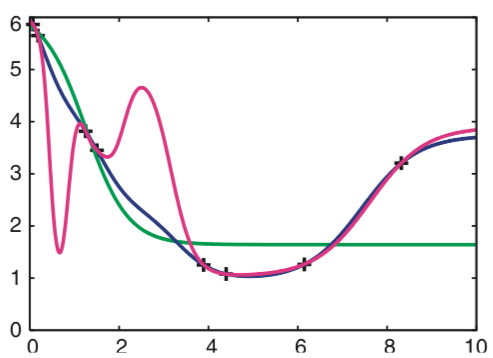
\includegraphics[width=0.6\linewidth]{graphics/krogh/krogh_overfitting.png}
    \caption*{Quelle: \textcite{Krogh2008}}
%\end{wrapfigure}
\end{figure}

Während die Problematik des Overfitting aus anderen Bereichen bereits bekannt ist, scheinen neuronale Netzwerke besonders anfällig für eine solche Überparametrierung. Würden wir ein Modell entwickeln, welches anhand 20 Merkmalen (20 Eingabewerte) mit Hilfe einer verstecken Schicht von 10 Neuronen erkennen soll, ob es sich um einen Hund oder eine Katze handelt, so würden 221 Parameter geschaffen. Jeder der 20 Eingabewerte wird durch ein Gewicht mit den 10 Neuronen aus der versteckten Schicht verbunden ($10 * 20 = 200$ Parameter). Jedes dieser Neuronen hat einen Threshold (10 Parameter) und ist mit dem Ausgabeneuron verknüpft (10 Parameter). Das Ausgabeneuron selbst hat auch wieder einen Threshold (1 Parameter). Wird dieses Modell mit 221 Parametern nun mit Hilfe von nur 100 Trainingsdatensätzen trainiert, so kann es diese problemlos auswendig lernen. Das Modell kann auf neuen Datensätzen nicht oder nur schlecht generalisieren und wird somit eine hohe Varianz aufweisen~\autocite{Krogh2008}.

Um ein solches Overfitting zu verhindert stehen diverse Techniken zur Verfügung. Eine beliebte Regularisierungstechnik ist es, eine sogenannte Dropout Schicht in das Netzwerk einzubringen. Diese Dropout Schicht deaktiviert während dem Training zufällige Neuronen. Dies hat zur Folge, dass während dem Training Teile des Netzwerks trainiert werden\footnote{Die genaue Funktionsweise einer Dropout Schicht ist für diese Arbeit nicht relevant, kann aber bei Bedarf in \textcite{Goodfellow2016} nachgelesen werden.}~\autocite{Goodfellow2016}.  

Um Over- respektive Underfitting zu erkennen, ist es also wichtig, ein neuronales Netzwerk an Daten zu testen, welche nicht zum Training verwendet wurden~\autocite{Krogh2008}.

\subsection{Long-Short-Term-Memory Netzwerke}

Menschen starten ihren Denkprozess nicht jede Sekunde von neuem. Beim Lesen wird jedes Wort aufgrund des Verständnisses des vorherigen Wortes verstanden. Gedanken sind persistent. Genau solche persistenten Gedanken sind mit den bisherigen Ansätzen für Neuronale Netze nicht modellierbar. Hier kommen Recurrent Neural Networks (kurz RNN) ins Spiel. Recurrent Neural Networks sind Neuronale Netzwerke mit integrierten Schlaufen~\autocite{Olah2015}. 

In Abbildung \ref{rnn1} wird ein RNN mit einer Schlaufe dargestellt. Daneben ist dasselbe Netzwerk in einer anderen, ausgerollten Weise zu sehen. Die Abbildung verdeutlicht, wie Informationen von einem Neuron zum anderen fliessen können. Mit diesem Informationsfluss von Neuron zu Neuron werden die Resultate jeweils von den vorhergehenden Neuronen beeinflusst. Damit wird eine Art Kurzzeitgedächtnis geschaffen, welches dem Neuronalen Netzwerk erlaubt mit Kontextinformationen zu arbeiten~\autocite{Olah2015}.
\begin{figure}[H]
    \captionsetup{width=.9\linewidth}
    \caption[Informationsfluss durch ein Recurrent Neural Network]{Informationsfluss durch ein Recurrent Neural Network dargestellt als Schlaufe (links) und als Sequenz (rechts)}
    \label{rnn1}
    \centering
    \vspace{0.2cm}
    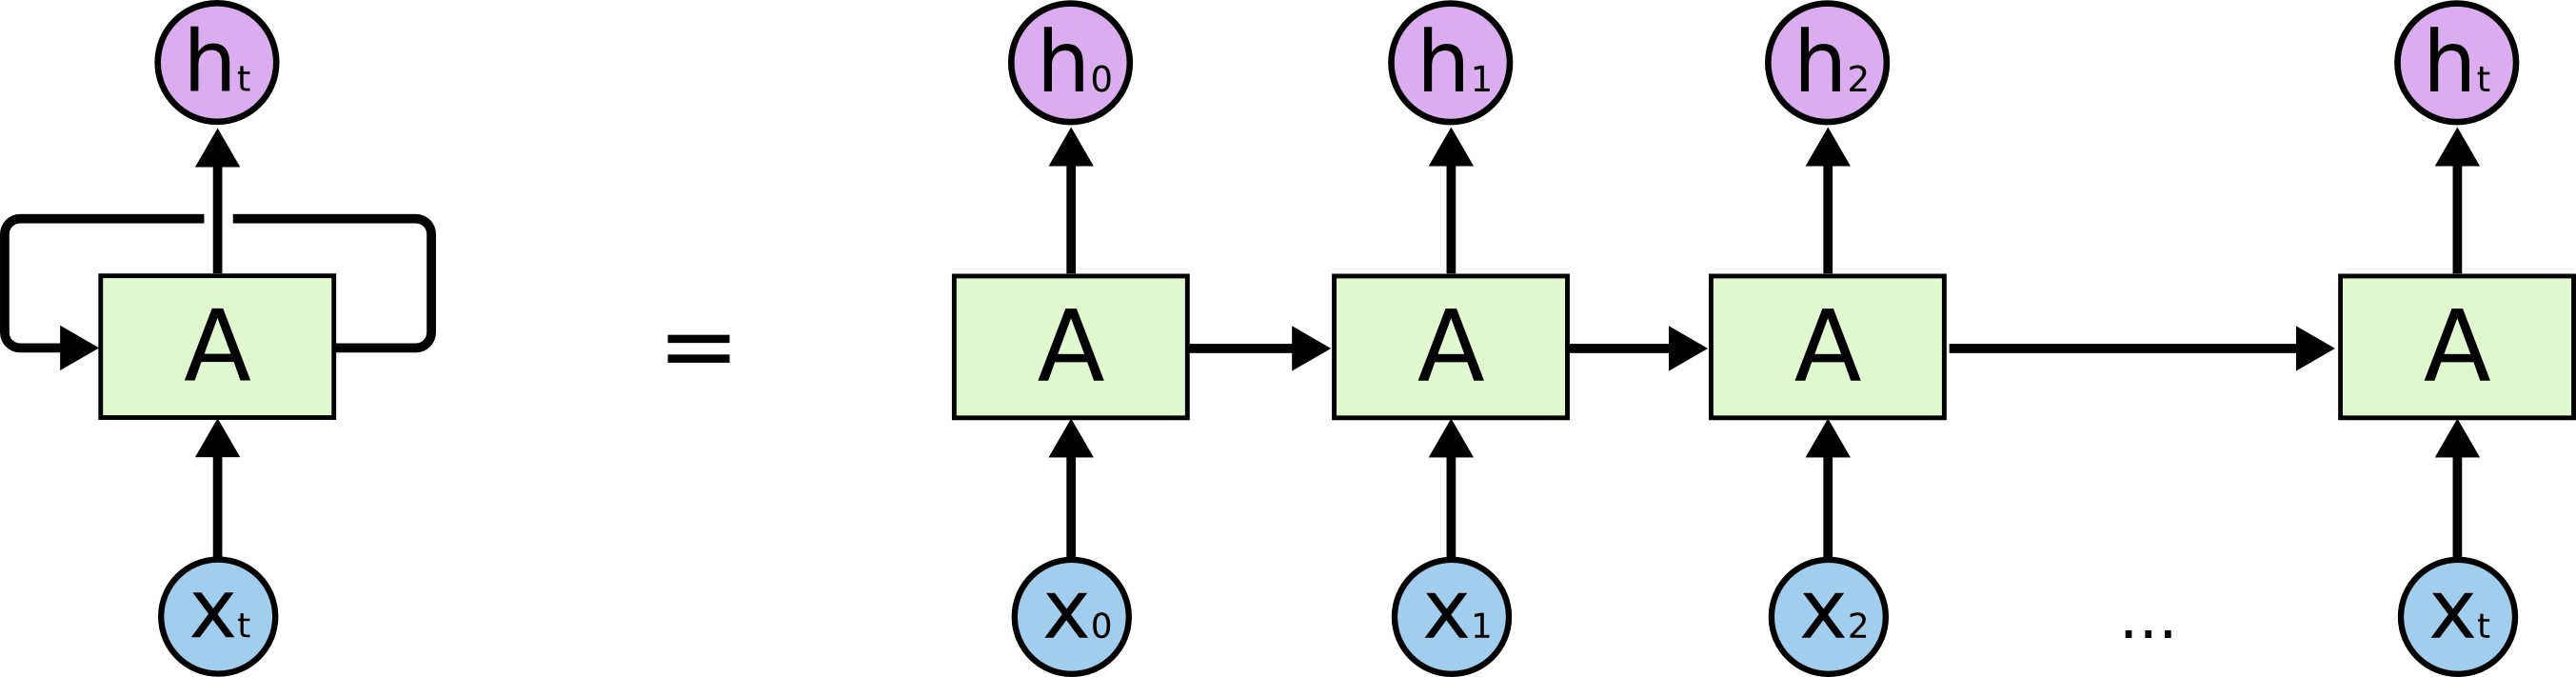
\includegraphics[width=0.6\textwidth]{graphics/rnn1.png}\\
    \vspace{0.3cm}
    \caption*{Quelle: \textcite{Olah2015}}
\end{figure}

Ein Problem von RNN ist, dass nur ein Kurzzeitgedächtnis zur Verfügung steht. Liegen Informationen länger zurück, sprich der Abstand zwischen den beiden relevanten Neuronen ist zu gross, gehen diese Informationen verloren. Eine Lösung für diese Problematik bieten Long-Short-Term-Memory (kurz LSTM) Netzwerke. Diese Spezialform von Recurrent Neural Networks arbeitet mit sogenannten Gates, um zu regulieren, wie viel Kontextinformationen behalten oder vergessen werden sollen. Mit vier solchen Gates, bestehend aus einem Neural Network Layer und einer Pointwise Operation (vgl. Abbildung \ref{lstm1}), ist ein LSTM Netzwerk in der Lage, nicht nur ein Kurz- sondern auch ein Langzeitgedächtnis aufzubauen~\autocite{Olah2015}.\todo{Punkt am schluss von Abbildungsbeschriftungen oder nicht? Einheitlich!}
\begin{figure}[H]
    \captionsetup{width=.9\linewidth}
    \caption[Veranschaulichung des Informationsflusses eines LSTM Netzwerk]{Veranschaulichung des Informationsflusses eines LSTM Netzwerk mit seinen vier internen Schichten}
    \label{lstm1}
    \centering
    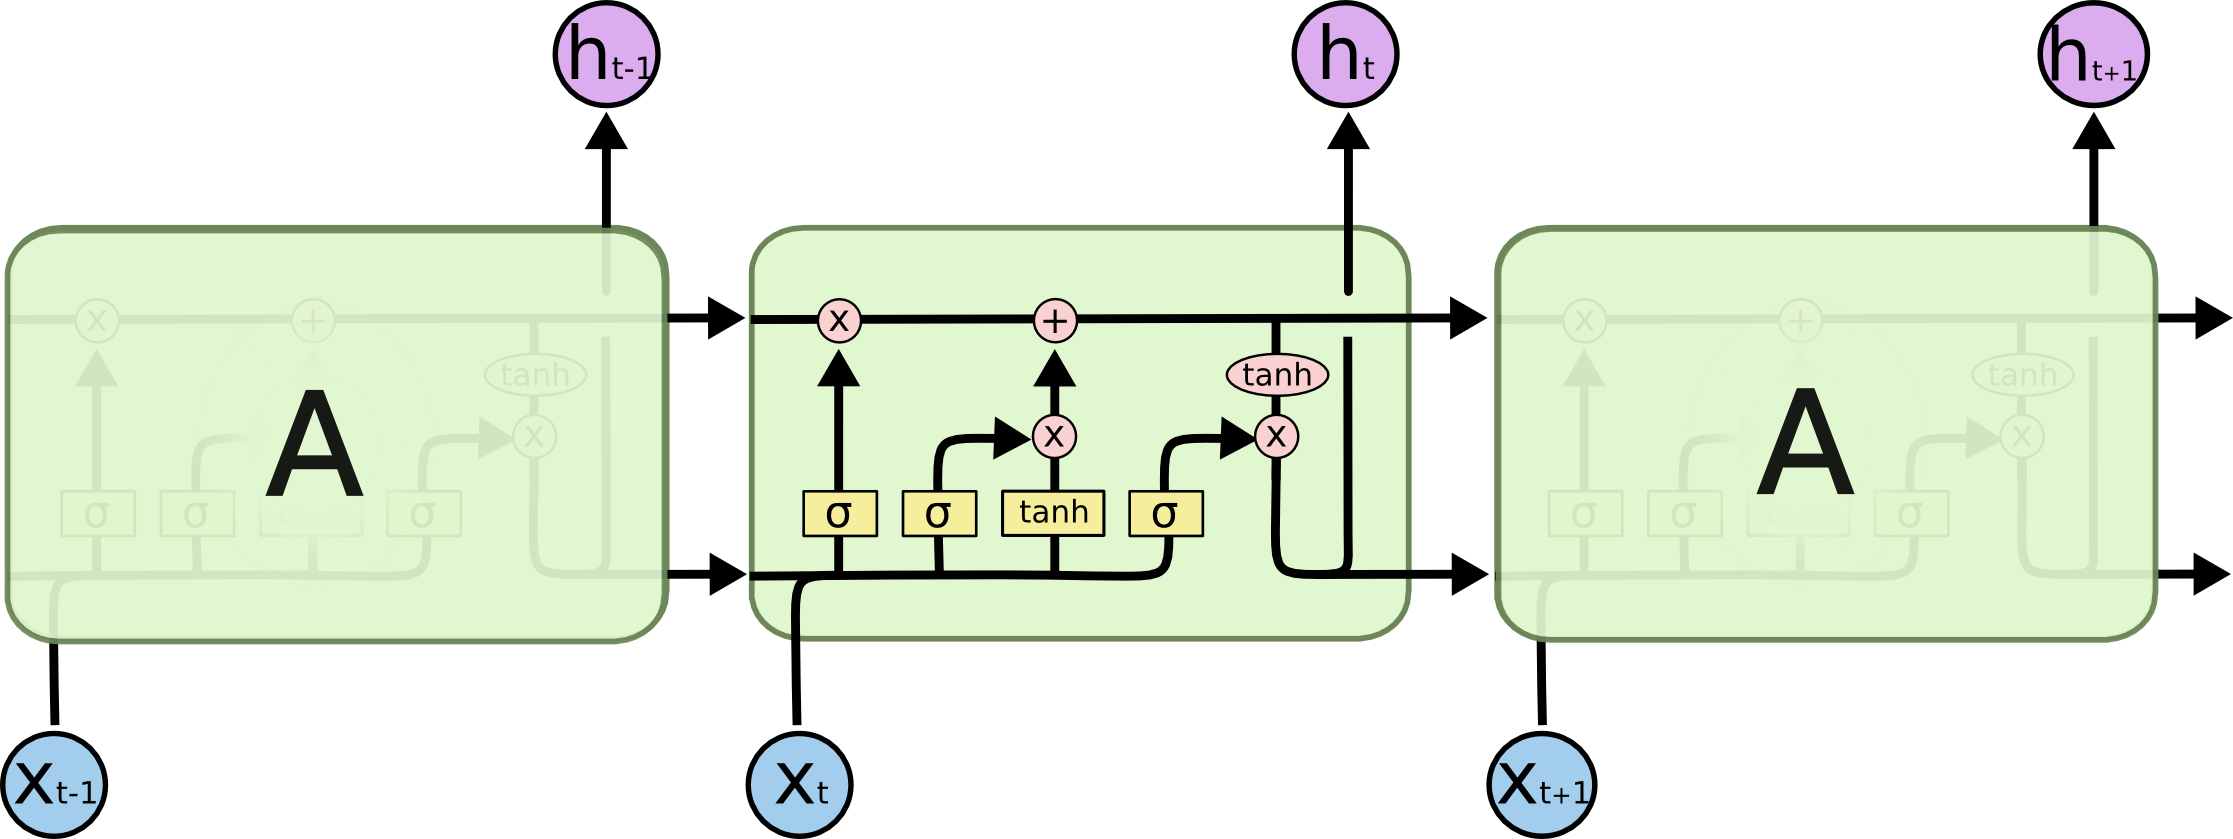
\includegraphics[width=0.6\textwidth]{graphics/lstm.png}\\
    \vspace{0.5cm}
    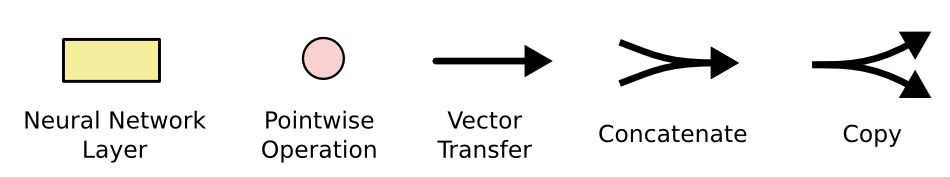
\includegraphics[width=0.6\textwidth]{graphics/lstm-notation.png}\\
    \vspace{0.1cm}
    \caption*{Quelle: \textcite{Olah2015}}
\end{figure}

Recurrent Neural Networks wurden in der Vergangenheit sehr erfolgreich für viele Aufgaben, wie beispielsweise die Spracherkennung, Sprachmodellierung, maschinelle Übersetzung sowie Bilderkennung, angewendet. In den meisten Fällen wurden dabei LSTM Netzwerke angewendet, da die Resultate um ein Vielfaches besser ausfallen als mit herkömmlichen RNNs~\autocite{Olah2015}.

LSTM Netzwerke sind für diese Arbeit besonders zur Texterkennung und Rechtschreibkorrektur interessant. Diese beiden Techniken werden im Prototypen der Rechnungsindexierung verwendet.

\subsection{Texterkennung}

Ein wichtiger Bestandteil des Prototypen zur Indexierung von Rechnungen ist die Erkennung von Texten, in Druckbuchstaben oder Handschrift, auf Rechnungen. Die erkannten Texte bilden die Grundlage für jegliche digitale Verarbeitung der Rechnungen.

Die herkömmliche Feature-detection in Texterkennungssoftware wird immer mehr mit künstlicher Intelligenz ersetzt. \textcite{Neuberg2017} beschreibt wie Dropbox künstliche Intelligenz anwendet, um Texte aus Fotografien von Dokumenten durchsuchbar zu machen. Zur Anwendung kommen dabei verschiedene Techniken aus dem Bereich der künstlichen Intelligenz: \textit{Convolutional Neural Network}\footnote{Ein Convolutional Neural Network ist eine Spezialform eines neuronalen Netzwerks bei welchen, etwas vereinfacht ausgedrückt, viele Kopien des gleichen Neurons zum Einsatz kommen\autocite{Olah2014}.} (CNN),  Long-Short-Term-Memory (LSTM) Netzwerke, Connectionist Temporal Classification\footnote{Connectionist Temporal Classification ist ein Konzept aus dem Training von neuronalen Netzwerken, welches vor allem in der Handschrifterkennung Verwendung findet. Dabei wird eine spezielle Trainingsfunktion verwendet, durch welche die Positionierung von Buchstaben generalisiert und somit der Lernprozess des neuronalen Netzwerks vereinfacht werden kann~\autocite{Scheidl2018}.} (CTC) und weitere~\autocite{Neuberg2017}.

Auch die Texterkennungssoftware Tesseract, welche ursprünglich als Forschungsprojekt im HP Lab entwickelt wurde und seit 2005 als Open Source Software zur freien Verfügung steht, verwendet seit Version 4 künstliche Intelligenz~\autocite{Smith2007}. So wurde die Feature-detecion durch ein LSTM Netzwerk mit mehr als 100 Schichten ersetzt. Die Texterkennung konnte so nicht nur qualitativ stark verbessert werden, sondern ist auch schneller als zuvor. Doch auch nach den Verbesserungen sind die Ergebnisse nicht perfekt und müssen fallspezifisch optimiert werden~\autocite{O.V.2018, O.V.2018a}.

\subsection{Word embedding}
\label{chap:embedding}

Neuronale Netzwerke funktionieren mit Zahlen. Damit auch Wörter und ganze Sätze von solchen Netzwerken verarbeitet werden können, muss eine geeignete Repräsentation von Wörtern durch Zahlen gefunden werden. Der Prozess, mit welchem ein Wort in eine zahlen-basierte Repräsentation gebracht wird, nennt sich Word embedding~\autocite{Olah2014b}.

Die ersten Word embeddings wurden von \textcite{Bengio2001} eingeführt. Trotz des schon fortgeschrittenen Alters dieses Forschungsgebiet ist es noch immer hoch interessant und in voller Fahrt~\autocite{Olah2014b}.

\begin{wrapfigure}{r}{0.5\textwidth} 
    \captionsetup{width=.9\linewidth}
    \caption[Modulares Netzwerk zur Validierung von 5-Grammen]{Modulares Netzwerk zur Validierung von 5-Grammen mit einer Word embedding Funktion ($W$) und einem Neuronalen Netzwerk ($R$)}
    \label{wordembeddingtraining}
    \centering
    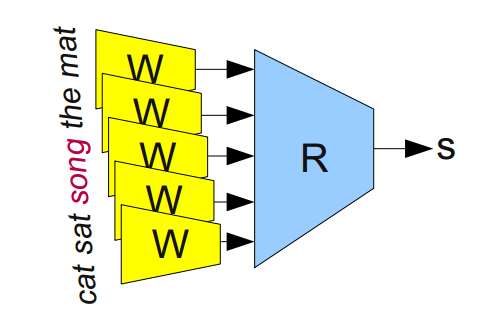
\includegraphics[width=0.48\textwidth]{graphics/wordembeddingtraining.png}
    \caption*{Quelle: \textcite{Olah2014b}}
\end{wrapfigure}
Technisch gesehen ist ein Word embedding eine parametrierte Funktion, welche Wörter einer bestimmten Sprache in einen hoch-dimensionalen Vektor (typischerweise 200-500 Dimensionen) transformiert. Um diese hoch komplexe Funktion zu definieren, kommt, wie bei den Neuronalen Netzwerken, Machine Learning zum Einsatz. \textcite{Olah2014b} beschreibt in seinem Artikel ein Beispiel, bei welchem eine solche Word embedding Funktion trainiert wird. Die Resultate aus dem Word embedding werden in ein Neuronales Netzwerk zur Prüfung eines 5-Grammes gespiesen und dann das Gesamtkonstrukt trainiert (vgl. Abbildung \ref{wordembeddingtraining})~\autocite{Olah2014b}.

Um sich Word embeddings besser vorstellen zu können, zieht \textcite{Olah2014b} zwei verschiedene Möglichkeiten der Visualisierung heran.

Die erste Visualisierung bedient sich dem t-SNE\todo{Beschreiben} Algorithmus um die hoch-dimensionalen Vektoren in einem zweidimensionalen Diagramm darzustellen. In einem solchen Diagramm ist klar zu erkennen, dass ähnliche Wörter nahe zusammen sind (vgl. Abbildung \ref{wordembeddingtsne})~\autocite{Olah2014b}.
\begin{figure}[H]
    \centering
    \captionsetup{width=.9\linewidth}
    \caption[t-SNE Darstellung eines Word embeddings]{t-SNE Darstellung eines Word embeddings, um zu verdeutlichen, dass ähnliche Wörter ähnliche Vektoren aufweisen}
    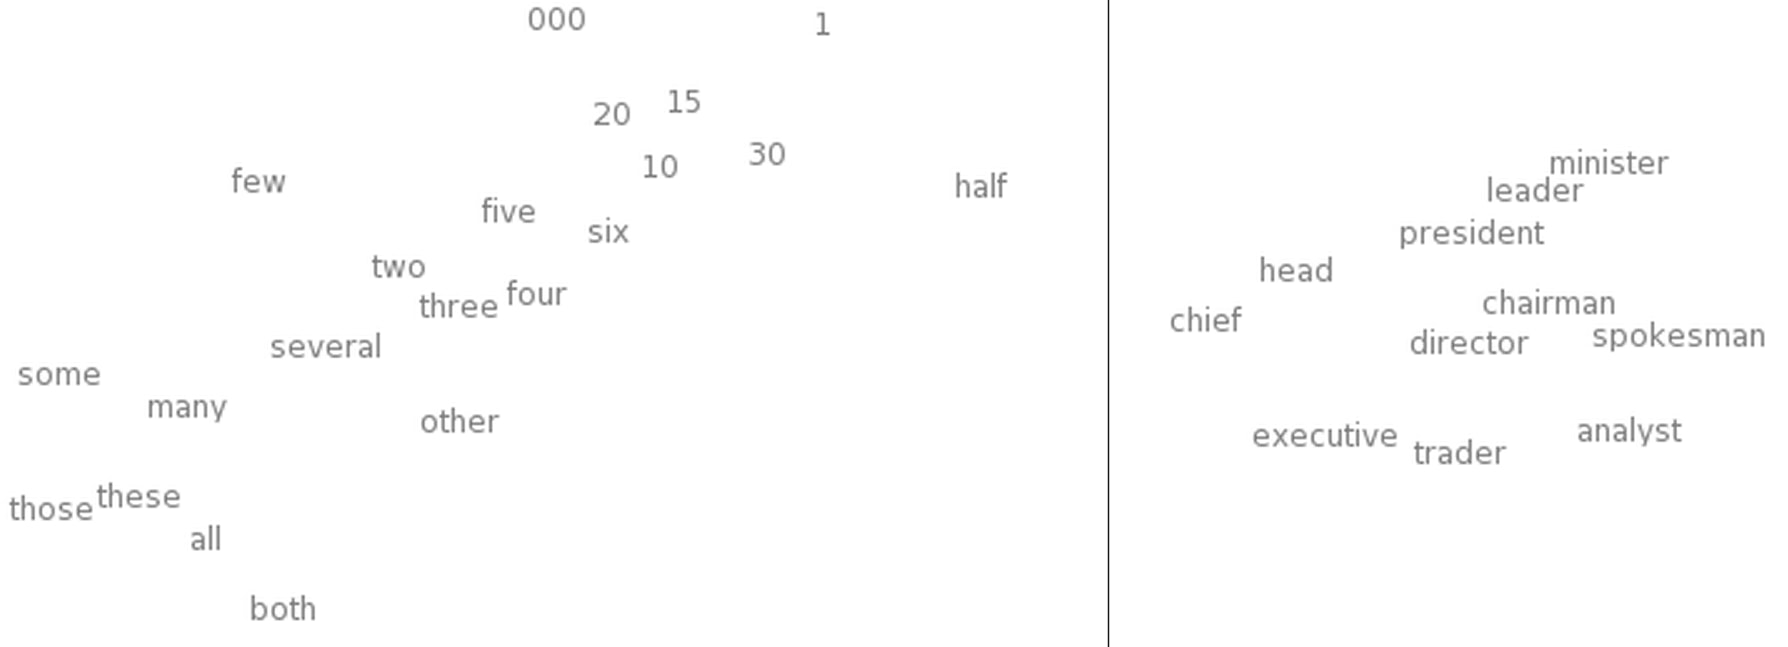
\includegraphics[width=\textwidth]{graphics/wordmebeddingtsne.jpg}
    \caption*{Quelle: \textcite{Turian2010} in \textcite{Olah2014b}}
    \label{wordembeddingtsne}
\end{figure}

Die zweite Visualisierung listet in einer Tabelle (vgl. Tabelle \ref{wordembeddingtable}) für sechs Wörter die nächsten Embeddings, sprich mit den mathematisch nächsten Vektoren, auf. So werden beispielsweise unter dem Titel \textit{FRANCE} neben \textit{EUROPA} diverse weitere Länder aufgelistet.
\begin{table}[H]
\centering
    \captionsetup{width=.9\linewidth}
    \caption[Ähnlichkeit von sechs Word-Embeddings]{Sechs Ausgangswörter mit den ihnen ähnlichsten Word embeddings, sprich mit den mathematisch nächsten Vektoren}
    \label{wordembeddingtable}
    \renewcommand{\arraystretch}{1.25}
    \setlength{\tabcolsep}{3pt}
    \footnotesize
    \begin{tabular}{ | l | l | l | l | l | l |}
    \hline
    \rowcolor{ccc} FRANCE & JESUS & XBOX & REDDISH & SCRATCHED & MEGABITS \\ \hline
    AUSTRIA & GOD & AMIGA & GREENISH & NAILED & OCTETS \\ \hline
    BELGIUM & SATI & PLAYSTATION & BLUISH & SMASHED & MB/S \\ \hline
    GERMNAY& CHRIST & MSX & PINKISH & PUNCHED & BIT/S \\ \hline
    ITALY & SATAN & IPOD & PRUPLISH & POPPED & BAUD \\ \hline
    GREECE & KALI & SEGA & BROWNISH & CRIMPED & CARATS \\ \hline
    SWEDEN & INDRA & PS\textit{NUMBER} & GREYISH & SCRAPED & KBIT/S \\ \hline
    NORWAY & VISHNU & HD & GRAYISH & SCREWED & MEGAHERTZ \\ \hline
    EUROPE & ANANDA & DRAMCAST & WHITISH & SECTIONED & MEGAPIXELS \\ \hline
    HUNGARY & PARVATI & GEFORCE & SILVERY & SLASHED & GBIT/S \\ \hline
    SWITZERLAND & GRACE & CAPCOM & YELLOWISH & RIPPED & AMPERES \\ \hline
    \end{tabular}
    \caption*{Quelle: \textcite{Collobert2011} in \textcite{Olah2014b}}
\end{table}

Sowohl Abbildung \ref{wordembeddingtsne} als auch Tabelle \ref{wordembeddingtable}, zeigen die Stärke von Word embeddings auf. Ähnliche Wörter werden mit ähnlichen Vektoren versehen und so wird eine komplexe Landschaft von zusammengehörigen Wörtern gebildet. Da somit zwei Synonyme ein ähnliches Word embedding aufweisen, verändert sich der Input-Vektor eines nachfolgenden neuronalen Netzwerks durch den Austausch dieser nur geringfügig. Somit muss dieses nachfolgende neuronale Netzwerk nicht für alle Wörter der Welt trainiert werden, sondern kann auf die Generalisierung durch das Word embedding aufbauen~\autocite{Olah2014b}.

Word embeddings sind zu einem extrem wichtigen Baustein bei der Verarbeitung von Natürlichen Texten geworden. Neben Input und Output Repräsentationen bei NLP Tasks können Word embeddings auch Output Repräsentationen in der Bilderkennung sein~\autocite{Olah2014b}. 

Für den Prototypen bilden Word embeddings eine wichtige Grundlage. Durch diese Technik können die in den Rechnungen enthaltenen Wörter und Sätze in eine generalisierte, durch Neuronale Netzwerke verarbeitbare Form gebracht werden.

\subsection{Korrektur von Rechtschreibung und Grammatik}
\label{chap:grammar-correction}

Trotz grossem Fortschritt, nicht zuletzt dank der Verwendung von künstlicher Intelligenz, im Bereich der Texterkennung, werden Texte nicht zu 100\% korrekt erkannt. So schleichen sich falsch erkannte Buchstaben ein, welche nicht nur Wörter, sondern auch ganze Sätze bedeutungslos machen. Um solche Fehler zu korrigieren, wird auf die Rechtschreibung- und Grammatik-Korrektur zurückgegriffen. Während diverse Korrekturprogramme regelbasierte Software anwenden, wurde auch in diesem Bereich bereits erfolgreich künstliche Intelligenz angewandt.\todo{Quelle}

Mit Hilfe der in einem vorherigen Kapiteln eingeführten Technik des Word embeddings und von LSTM Netzwerken lässt sich diese Problematik angehen. So kann ein modulares Netzwerk aus Word embeddings und mehreren LSTM Schichten verwendet werden, um eine Rechtschreibkorrektur vorzunehmen. So beschreibt \textcite{Weiss2016} in seinem Blog, wie mit einem einfachen neuronalen Netzwerk, bestehend aus nur 4 LSTM und 4 Dropout Schichten, bereits erfolgreich Rechtschreibfehler korrigiert werden können. 

% can't use wrapfigure here as otherwise the next sections wraps too
\begin{figure}[H] % wrapfigure}{l}{0.5\textwidth}
    \centering
    \captionsetup{width=.9\linewidth}
    \caption{Vergleich der Erfolgsrate bei der Prüfung von 418 Textsnippets}
    \label{deepgrammar}
    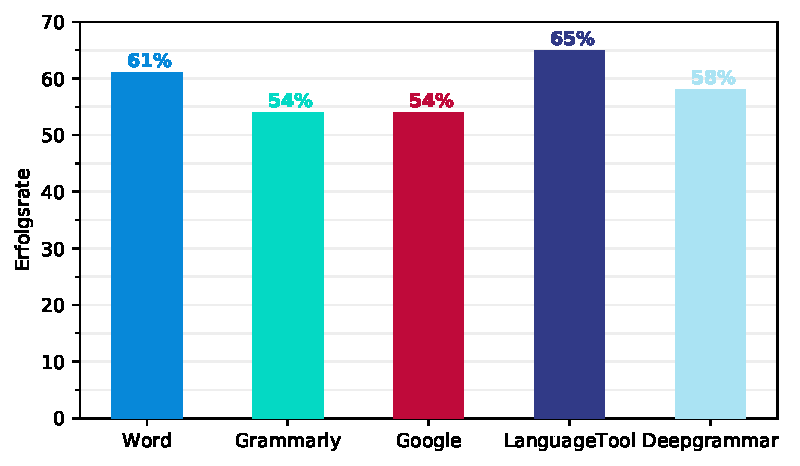
\includegraphics{graphics/matplot/grammar-tools.pdf}
    \caption*{Quelle: \textcite{Mugan}}
\end{figure} %wrapfigure}
Nicht nur zur Korrektur von Rechtschreibfehlern ist ein neuronales Netzwerk anwendbar, sondern auch zur Grammatikprüfung. So kann unter deepgrammar.com ein Experiment gefunden werden, bei welchem ein neuronales Netzwerk zur Grammatikprüfung angewendet wird. Die Resultate, welche in der Abbildung \ref{deepgrammar} zu sehen sind, sind erstaunlich. Obwohl DeepGrammar erst seit einem Jahr existiert und dabei von nur einer Person entwickelt wurde, funktioniert das Netzwerk beinahe so gut wie \textit{Microsoft Word}\footnote{Microsoft Word ist ein Programm zur Textverarbeitung und Dokumenterstellung von Microsoft~\autocite{MicrosoftCorporation2018}.} oder \textit{Language Tool 3.1}\footnote{\enquote{LanguageTool ist eine Software zur Textprüfung [...]}~\autocite{LanguageTool2018}.} und sogar besser als \textit{Grammarly}\footnote{Grammarly verspricht präzise, kontextabhängige Korrekturen von Texten~\autocite{GrammarlyInc.2018}.} und \textit{Google Docs}\footnote{Google Docs ist eine Online-Lösung zur Textverarbeitung von Google~\autocite{GoogleLLC2018}.}~\autocite{Mugan}.

% TODO: Mugan erwähnt eine bessere Studie. In der Thesis diese verwenden, da Zahlen aus DeepGrammar nicht 100% korrekt sind https://arxiv.org/pdf/1807.01270.pdf

Ein weiterer grosser Vorteil von neuronalen Netzwerken zur Fehlerkorrektur erwähnt \textcite{Mugan2018} in einer persönlichen Kommunikation. Das Neuronale Netzwerk kann auf das Domänenspezifische Lexikon trainiert werden. Das Netzwerk kann beispielsweise mit medizinischen Begriffen aus den Rechnungen trainiert werden, so dass die Resultate des in dieser Arbeit entwickelten Prototypen noch besser werden~\autocite{Mugan2018}.

\subsection{Informationsextraktion aus natürlichen Texten}
\label{chap:ner}

% https://en.wikipedia.org/wiki/Named-entity_recognition
% https://en.wikipedia.org/wiki/Medical_classification

Informationsextraktion beschreibt das Themengebiet rund um die Extraktion von strukturierten Informationen aus unstrukturiertem oder halb-strukturiertem Text. In diesem Kapitel werden einige Techniken aus diesem Themengebiet erläutert und deren Ein\-satz\-mög\-lich\-keit für die Entwicklung des Prototypen diskutiert.

Eine \textit{Regular Expression} (kurz RegEx) ist ein Ausdruck, welcher eine Zeichenkette beschreibt. Diese Ausdrücke funktionieren ähnlich wie arithmetische Ausdrücke: Es werden Operatoren verwendet, um mehrere Ausdrücke zu einem komplexeren Ausdruck zusammenzufassen~\autocite{Xiao2004}.

\textcite{Xiao2004} beschreibt als einfaches Beispiel den Ausdruck \texttt{[a,p]m [0-9]+:[0-9]+} um Zeitangaben wie AM 12:45 zu extrahieren. Dieses Beispiel zeigt einerseits die Einfachheit dieser Technik aber auch die Grenzen. 12:45 AM wird beispielsweise nicht erkannt, da AM hier nach anstelle vor der Uhrzeit steht. 

Ein weiterer Nachteil von Regular Expressions ist, dass Kontextinformationen nicht be\-rück\-sich\-tigt werden. Folgendes Beispiel von \textcite{Xiao2004} zeigt dies auf. Der Ausdruck \texttt{[0-9]+} ist zwar in der Lage aus dem Text \texttt{100\$} die Zahl \texttt{100} zu extrahieren, allerdings geht die Information, dass es sich hier um einen Geldbetrag handelt, verloren.

Um eine hohe Präzision bei der Informationsextraktion zu ermöglichen, sollten Regular Expressions also nur mit Vorsicht und in Kombination mit anderen Techniken verwendet werden~\autocite{Xiao2004};

Named Entity Recognition and Classification (kurz NERC oder NER), beschreibt das erkennen und kategorisieren von Entitäten, sprich Wörter oder Wortgruppen aus natürlichen Texten~\autocite{Nadeau2007}.

Der Begriff \textit{Named Entity} wurde bei der Formulierung der Aufgabenstellung der sechsten Message Understanding Conference im Jahre 1995 definiert~\autocite{Borthwick1998}. So wurde bereits damals erkannt, dass die Extraktion von Namen von Personen, Organisationen oder Lokationen, nummerischen Ausdrücken, Daten und Prozent-Ausdrücken wichtig ist~\autocite{Nadeau2007}.

Für die Named Entity Recognition and Classification stehen einige freie Softwarelösungen zur Verfügung. So veröffentlicht beispielsweise Stanford eine Java Implementierung und SpaCy, eine Sammlung von Natural Language Processing Software, beinhaltet eine Implementierung in Python~\autocite{StanfordNLPGroup, ExplosionAI}.

Die Anwendung von NERC ist für das Fallbeispiel äusserst interessant. Die Erkennung von Namen von Personen ist hilfreich zur Erkennung des Patienten und des Leistungserbringers. Weiter hilft die Erkennung von Daten der Ermittlung des Behandlungsdatums und nicht zuletzt kann durch die Erkennung und Klassifizierung von nummerischen Ausdrücken der Gesamtbetrag sowie die Beträge einzelner Positionen ermittelt werden.

Die letzte Technik, welche in diesem Kapitel erläutert wird, ist das \textit{Part of Speech Tagging} (kurz PoS-Tagging). Beim PoS-Tagging werden Wörter und Satzzeichen ihren Wortarten (Nomen, Adjektive, etc.) zugewiesen~\autocite{Xiao2004}.

Die grösste Herausforderung beim PoS-Tagging sind Wörter welche verschiedenen Wortgruppen zugewiesen werden könnten. Beispielsweise kann das Wort \textit{widerwillig} im Satz \textit{Sie nannten den Täter widerwillig.} als Adjektiv oder Adverb aufgefasst werden und somit die Bedeutung des Satzes vollkommen verändern~\autocite{Volk}.

% Es gibt diverse Arten von Implementierung des PoS-Tagging, welche in regelbasierte, stochastische und neuronale Verfahren unterteilt werden können. Ein weit verbreiteter Ansatz ist die Verwendung von Hidden Markov Modellen. Ein Hidden Markov Modell ist ein stochastisches Modell, welches Zustände mit übergangswahrscheinlichkeiten modelliert.

% Die Verwendung von PoS-Tagging kann bei Rechnungen mit einem Prosatext von Vorteil sein. Wie viele relevante Informationen in Prosatexten von Rechnungen verborgen sind, muss sich aber erst noch zeigen.

% Die beschriebenen Techniken bieten eine gute Grundlage um damit eine erste Implementierung eines Prototypen zur Rechnungsindexierung zu beginnen.

\subsection{Transfer Learning}
\label{chap:transfer-learning}

Transfer Learning beschreibt das Vorgehen, bei welchem das Gelernte aus einer Aufgabe genutzt wird, um das Lernen für eine andere Aufgabe zu vereinfachen~\autocite{Goodfellow2016}.

Beim Transfer Learning wird ein Modell verwendet, um zwei oder mehr verschiedene Aufgaben zu lösen. Es wird dabei angenommen, dass die Vorhersagen für eine Aufgabe aufgrund ähnlicher Kriterien getroffen werden wie für jene einer anderen Aufgabe. Dies ist typischerweise dann der Fall, wenn die Eingabewerte eines Modells gleich oder ähnlich sind, sich die Art der gesuchten Ausgabewerte aber unterscheidet~\autocite{Goodfellow2016}.

Ein Beispiel für ein solches Transfer Learning ist, wenn ein Modell trainiert wird, Bilder von Hunden und Katzen zu klassifizieren. Dabei stehen viele Trainingsdaten zur Verfügung. Nun soll ein Modell entwickelt werden, welches Bilder von Ameisen und Wespen klassifiziert. Sind nun für die zweite Aufgabe nur wenige Trainingsdaten verfügbar, so ist es denkbar, das Modell aus erster Aufgabe als Grundlage zu verwenden. Da viele visuelle Repräsentationen grundlegende Eigenschaften wie Formen und Kanten teilen, kann die Wiederverwendung des trainierten Modells aus erster Aufgabe die Treffergenauigkeit in der zweiten Aufgabe stark erhöhen~\autocite{Goodfellow2016}.

Wird ein Modell, welches bereits für eine Aufgabe trainiert wurde, für eine zweite Aufgabe weiter trainiert, spricht man von Fine Tuning~\autocite{Goodfellow2016}.

Ursprünglich kommt das Transfer Learning aus dem Bereich der Computer Vision. Im Jahr 2018 präsentierten \textcite{Howard2018} sowie \textcite{Devlin2018} mit ULMFiT\footnote{Universal Language Model Fine-tuning, kurz ULMFiT, ist ein Ansatz, bei welchem ein Modell auf einem sehr grossen Datensatz trainiert wird. Dieses Modell kann nun für diverse Aufgaben im Gebiet des Natural Language Processing verwendet werden und verspricht bessere Ergebnisse als Ansätze ohne Transfer Learning\autocite{Howard2018}.} respektive BERT\footnote{Bidirectional Encoder Representations from Transformes, kurz BERT, ist eine neuartige Repräsentation von natürlicher Sprache. Mit diesem auf Transfer Learning basierten Ansatz konnte das Google AI Language Team in diversen NLP Aufgaben neue Bestresultate erzielen\autocite{Devlin2018}.} Ansätze, das Transfer Learning auch für Aufgaben im Gebiet des Natural Language Processing anzuwenden. Beide Ansätze versprechen die Reduktion der Menge benötigter Traingsdatensätze sowie die Verbesserung der resultierenden Modelle.

\subsection{Messkriterien zur Bewertung eines KI Systems}
\label{chap:metrices}

Um ein System objektiv zu Bewerten und mit anderen Ansätzen zu vergleichen, bedarf es Metriken. Folgend werden einige Metriken erläutert und ihre Anwendungsfälle diskutiert.

\subsubsection{Treffergenauigkeit}

Die Treffergenauigkeit, englisch Accuracy (kurz acc), ist die Metrik, welche wohl am meisten im Zusammenhang mit der künstlichen Intelligenz zu finden ist. Die Frage ist aber, ob diese Metrik für alle Anwendungsfälle geeignet ist~\autocite{TDSAccuracy}.

Die Treffergenauigkeit sagt aus, wie viele der Vorhersagen eines Systems der Wirklichkeit entsprechen. Die Formell lautet wie folgt~\autocite{TDSAccuracy}: 

$$Accuracy = 1 - \frac{False Positive + False Negative}{Total Records}$$

Die Confusion Matrix in Abbildung \ref{cm-sample} zeigt ein Beispiel mit einer Treffergenauigkeit von 0.99, respektive 99.9\%. Aus 1000 Datensätzen wurden 998 korrekt als Negativ klassifiziert. Ein Datensatz wurde korrekt als Positiv klassifiziert und ein Datensatz wurde fälschlicherweise als Negativ klassifiziert~\autocite{TDSAccuracy}.

\begin{figure}[H]
    \centering
    \captionsetup{width=.9\linewidth}
    \caption{Beispiel einer Confusion Matrix zur Veranschaulichung der Treffergenauigkeit}
    \label{cm-sample}
    \def\arraystretch{1.5}
    \arrayrulecolor{black}
    \begin{tabular}{llcc}
        \multicolumn{2}{l}{}                                                                       & \multicolumn{2}{c}{\textbf{Vorhersage / Klassifizierung}}   \\ \cline{3-4} 
        \multicolumn{1}{c}{\textbf{}}                               & \multicolumn{1}{l|}{}        & \multicolumn{1}{c|}{Negativ} & \multicolumn{1}{c|}{Positiv} \\ \cline{2-4} 
        \multicolumn{1}{l|}{\multirow{2}{*}{\textbf{Wirklichkeit}}} & \multicolumn{1}{l|}{Negativ} & \multicolumn{1}{c|}{998}    & \multicolumn{1}{c|}{0}       \\ \cline{2-4} 
        \multicolumn{1}{l|}{}                                       & \multicolumn{1}{l|}{Positiv} & \multicolumn{1}{c|}{1}       & \multicolumn{1}{c|}{1}       \\ \cline{2-4} 
    \end{tabular}
    \caption*{Quelle: \textcite{TDSAccuracy}}
\end{figure}

Eine Treffergenauigkeit von 99.9\% ist sehr gut. Das Modell könnte durchaus als sehr erfolgreich betrachtet werden. Diese Betrachtung ist aber abhängig vom Anwendungsfall des Modells. Wenn das Modell die Infektion mit einem hoch ansteckenden Virus ermitteln würde, so wäre eine Infektion unentdeckt geblieben. In diesem Fall wäre eine geringere Treffergenauigkeit des Modells besser, wenn dafür keine falsche negativ Vorhersagen vorhanden wären. Die Metriken der folgenden Kapitel könnten für diesen Anwendungsfall besser geeignet sein~\autocite{TDSAccuracy}.

\subsubsection{Genauigkeit}

Die Genauigkeit, English Precision, sagt aus, wie viele als positiv vorhergesagten Datensätze wirklich Positiv sind. Die Formell dazu lautet (vgl. Abbildung \ref{cm-precision})~\autocite{TDSAccuracy}: 

$$Precision = \frac{True Positive}{True Positive + False Positive} = \frac{True Positive}{Total Predicted Positive}$$

Die Genauigkeit bietet sich immer dann als gute Metrik an, wenn die Kosten eines False Positive hoch sind. Ein Beispiel dafür ist ein Spamfilter. Markiert der Spamfilter ein E-Mail fälschlicherweise als kein Spam, so ist dies kein grosses Problem. Der Anwender kann das E-Mail einfach selbst als Spam markieren. Markiert der Spamfilter jedoch ein E-Mail fälschlicherweise als Spam, so ist die Wahrscheinlichkeit hoch, dass der Anwender das E-Mail nie lesen wird~\autocite{TDSAccuracy}.

\begin{figure}[H]
    \centering
    \captionsetup{width=.9\linewidth}
    \caption[Confusion Matrix als Veranschaulichung der Genauigkeit]{Confusion Matrix als Veranschaulichung der Genauigkeit. Die blau hervorgehobenen Elemente bilden die Grundlage zur Berechnung der Genauigkeit.}
    \label{cm-precision}
    \def\arraystretch{1.5}
    \begin{tabular}{llcc}
        \multicolumn{2}{l}{}                                                                        & \multicolumn{2}{c}{\textbf{Vorhersage / Klassifizierung}}                                         \\ \cline{3-4} 
        \multicolumn{1}{c}{\textbf{}}                                & \multicolumn{1}{l|}{}        & \multicolumn{1}{c|}{Negativ}        & \multicolumn{1}{c|}{\cellcolor[HTML]{B5D0EE}Positiv}        \\ \cline{2-4} 
        \multicolumn{1}{l|}{}                                        & \multicolumn{1}{l|}{Negativ} & \multicolumn{1}{c|}{True Negative}  & \multicolumn{1}{c|}{\cellcolor[HTML]{B5D0EE}False Positive} \\ \cline{2-4} 
        \multicolumn{1}{l|}{\multirow{-2}{*}{\textbf{Wirklichkeit}}} & \multicolumn{1}{l|}{Positiv} & \multicolumn{1}{c|}{False Negative} & \multicolumn{1}{c|}{\cellcolor[HTML]{B5D0EE}True Positive}  \\ \cline{2-4} 
    \end{tabular}
    \caption*{Quelle: \textcite{TDSAccuracy}}
\end{figure}

\subsubsection{Sensitivität}

Die Sensitivität, English \textit{Recall}, sagt aus, wie viele wirklich positiven Datensätze als Positiv vorhergesagt werden. Die Formel zur Berechnung der Sensitivität lautet (vgl. Abbildung \ref{cm-recall})~\autocite{TDSAccuracy}: 

$$Precision = \frac{True Positive}{True Positive + False Negative} = \frac{True Positive}{Total Actual Positive}$$

Die Sensitivität ist immer dann relevant, wenn die Auswirkungen durch ein False Negative gross sind. Ein Beispiel dafür ist die Klassifizierung von Banktransaktionen auf Betrug. Wird eine nicht-Betrug Transaktion als Betrug markiert, so kann dies schnell abgeklärt und korrigiert werden. Wird jedoch eine Betrug Transaktion nicht als solche erkannt, so sind die finanziellen Auswirkungen gross~\autocite{TDSAccuracy}.

\begin{figure}[H]
    \centering
    \captionsetup{width=.9\linewidth}
    \caption[Confusion Matrix als Veranschaulichung der Sensitivität]{Confusion Matrix als Veranschaulichung der Sensitivität. Die blau hervorgehobenen Elemente bilden die Grundlage zur Berechnung der Sensitivität.}
    \def\arraystretch{1.5}
    \begin{tabular}{llcc}
        \multicolumn{2}{l}{}                                                                                                & \multicolumn{2}{c}{\textbf{Vorhersage / Klassifizierung}}                                                                \\ \cline{3-4} 
        \multicolumn{1}{c}{\textbf{}}                                & \multicolumn{1}{l|}{}                                & \multicolumn{1}{c|}{Negativ}                                & \multicolumn{1}{c|}{Positiv}                               \\ \cline{2-4} 
        \multicolumn{1}{l|}{}                                        & \multicolumn{1}{l|}{Negativ}                         & \multicolumn{1}{c|}{True Negative}                          & \multicolumn{1}{c|}{False Positive}                        \\ \cline{2-4} 
        \multicolumn{1}{l|}{\multirow{-2}{*}{\textbf{Wirklichkeit}}} & \multicolumn{1}{l|}{\cellcolor[HTML]{B5D0EE}Positiv} & \multicolumn{1}{c|}{\cellcolor[HTML]{B5D0EE}False Negative} & \multicolumn{1}{c|}{\cellcolor[HTML]{B5D0EE}True Positive} \\ \cline{2-4} 
    \end{tabular}
    \caption*{Quelle: \textcite{TDSAccuracy}}
    \label{cm-recall}
\end{figure}

\subsubsection{F\textsubscript{1}-Score}
\label{chap:f1-score}

Der F\textsubscript{1}-Score, auch F-Mass, vereint die Genauigkeit und die Sensitivität. Im Gegensatz zur Treffergenauigkeit lässt sich der Wert aber nicht durch ein Übermass an True Negatives beeinflussen, denn sie finden keine Beachtung bei der Berechnung. In den meisten Anwendungsfällen sind True Negatives nicht relevant. False Negatives und False Positives sind meist die Verursacher von potentiell verursachten Kosten. Der F\textsubscript{1}-Score wird mit folgender Formel berechnet~\autocite{TDSAccuracy}:

$$F_1=2 * \frac{\textnormal{Genauigkeit} * \textnormal{Sensitivität}}{\textnormal{Genauigkeit} + \textnormal{Sensitivität}}$$

Der F\textsubscript{1}-Score ist also eine gute Verbindung der Genauigkeit und der Sensibilität. Aufgrund der Vernachlässigung der True Negatives ist der F\textsubscript{1}-Score besonders bei ungleichmässig verteilten Klassen, sprich übermässig vielen True Negatives, sinnvoll~\autocite{TDSAccuracy}.

\subsubsection{Loss und Loss-Funktion}

Das sogenannte Loss, auch Kosten oder Fehler, zeigt, wie sehr eine Vorhersage von der Realität abweicht. Um das Loss zu berechnen, kommt die Loss-Funktion, auch Kosten- oder Fehler-Funktion, zur Anwendung. Wie genau die Loss-Funktion definiert wird, hängt von der Problemstellung ab. Bei einer Binären Klassifikation ist beispielsweise die Cross-Entropy-Loss–Function oder die Log-Loss–Function gängig~\autocite{TDSLoss}. 

Während dem Training ist das Loss, in diesem Fall die Differenz zwischen Vorhersage des Modells und den Trainingsdaten, die zu optimierende Grösse. Die Wahl der Loss-Funktion kann einen erheblichen Einfluss auf das Modell haben. Die Loss-Funktion wird während dem Training meist durch Regularisierungstechniken erweitert, um ein Overfitting zu verhindern~\autocite{Goodfellow2016}.

\subsubsection{Intersection over Union}

Um die Treffergenauigkeit, Genauigkeit und die Sensitivität zu berechnen, muss klar sein, ob eine Vorhersage eines Modells korrekt war oder nicht. Das bedeutet, es muss klar sein, ob es sich um einen True Positive, False Positive, True Negative oder False Negative handelt. 

Bei der Objekterkennung in Bildern ist dies aber nicht immer eindeutig zu sagen. Ein Modell zur Objekterkennung sagt eine Position eines Objektes, als umschliessendes Rechteck, sowie dessen Klasse vorher. Die Korrektheit der Klasse kann sehr einfach beurteilt werden. Entweder die Vorhersage stimmt mit der Erwartung überein oder nicht. Die Beurteilung der Korrektheit der vorhergesagten Position ist dagegen nicht eindeutig, wie dies Abbildung \ref{fig:iou-issue} verdeutlicht. Die Vorhersage des Modells trifft nicht exakt die Erwartung, doch deshalb ist die Vorhersage nicht falsch. Eine exakte Übereinstimmung des vorhergesagten und des erwarteten Rechtecks ist sehr unwahrscheinlich. Aus diesem Grund ist eine Metrik notwendig, die solche Ungenauigkeiten zulässt~\autocite{IoU}.

\begin{figure}[H]
    \captionsetup{width=.9\linewidth}
    \caption{TODO}
    \label{fig:iou-issue}
    \centering
    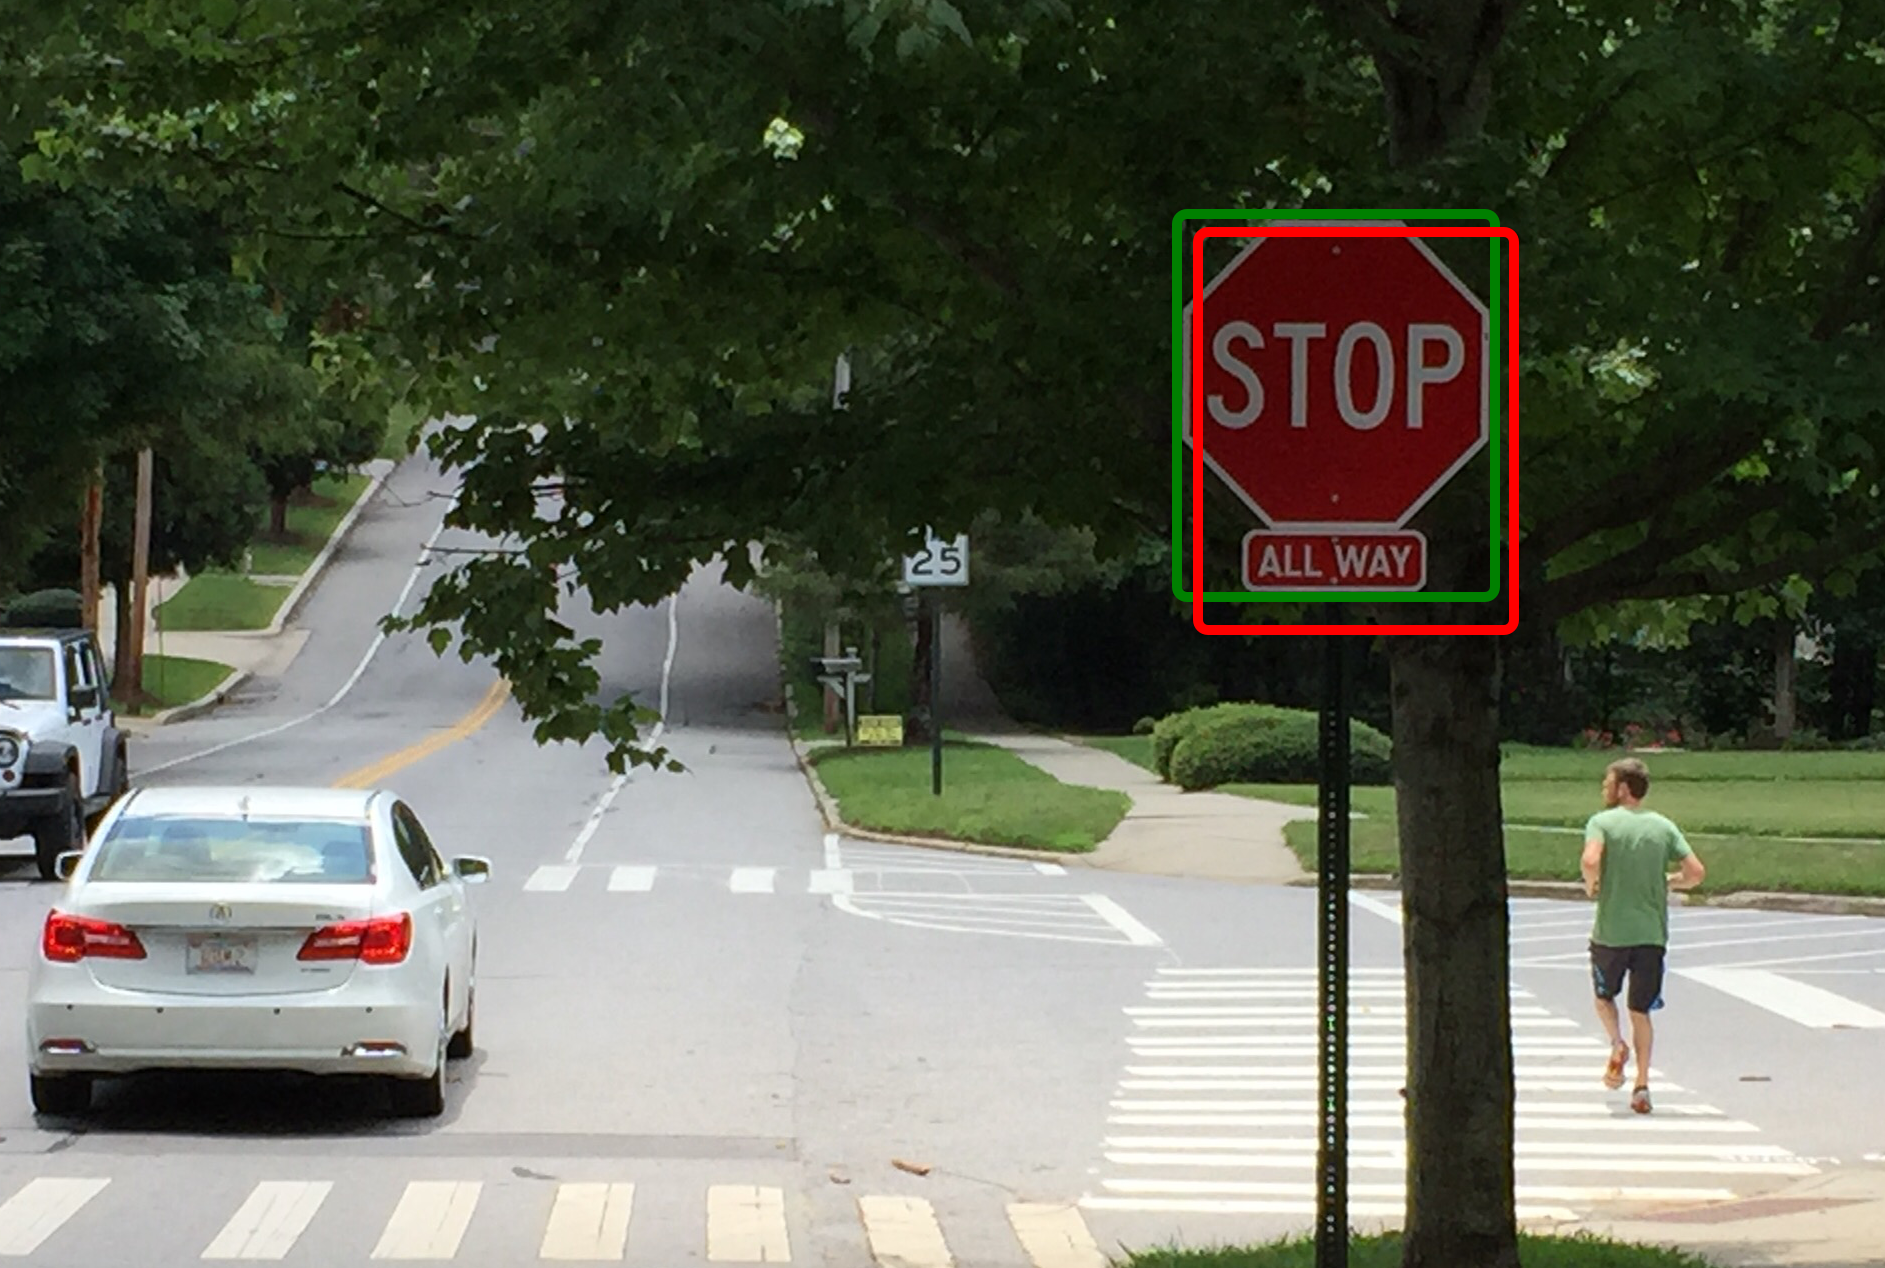
\includegraphics[width=0.6\textwidth]{graphics/iou/iou_issue.png}\\
    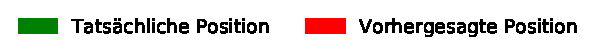
\includegraphics[scale=1]{graphics/matplot/iou_issue_legend.pdf}
    \caption*{Quelle: \textcite{IoU}}
\end{figure}

Intersection over Union, kurz IoU, ist ein solches Mass. Es stellt, wie es der Name bereits sagt, die Überlappung des vorhergesagten mit dem erwarteten Rechteck in das Verhältnis zur Vereinigung dieser~\autocite{IoU}:

$$IoU = \frac{
    \textnormal{Fläche der Überlappung} \hspace{10pt} 
\includegraphics[width=20pt]{graphics/iou/intersection.pdf}
}{
    \textnormal{Fläche der Vereinigung} \hspace{12pt} 
\includegraphics[width=20pt, align=t]{graphics/iou/union.pdf}
}$$

Die Beispiele aus Abbildung \ref{fig:iou-examples} verdeutlichen, dass das Mass gegen 1 tendiert, je exakter das vorhergesagte mit dem erwarteten Rechteck übereinstimmt. Es kann nun also beurteilt werden, wie genau die Vorhersage ist. Wird nun noch ein Schwellenwert definiert, ab welchem eine Vorhersage als Korrekt angesehen wird, so kann die Korrektheit der Vorhersage beurteilt werden. Die Wahl dieses Schwellenwerts ist sehr unterschiedlich. In Bilderkennungs-Wettbewerben sind Schwellenwerte zwischen 0.5 und 0.75 üblich. Auch wird teilweise ein Durchschnitt über mehrere Schwellenwerte verwendet~\autocite{IoU}.

\begin{figure}[H]
    \captionsetup{width=.9\linewidth}
    \caption{Beispiele des Intersection over Union Mass}
    \label{fig:iou-examples}
    \centering
    \begin{subfigure}[b]{0.3\linewidth}
        \centering
        \caption*{$IoU=0.4034$}
        % rescaling doesn't matter as there is no text in the graphics
        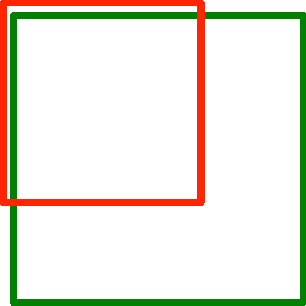
\includegraphics[width=0.5\linewidth]{graphics/iou/iou_examples/1.pdf}
        \caption*{Schlecht} 
        \vspace{2ex}
    \end{subfigure}%% 
    \begin{subfigure}[b]{0.3\linewidth}
        \centering
        \caption*{$IoU=0.7330$} 
        % rescaling doesn't matter as there is no text in the graphics
        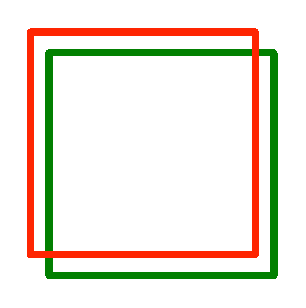
\includegraphics[width=0.5\linewidth]{graphics/iou/iou_examples/2.pdf}
        \caption*{Gut} 
        \vspace{2ex}
    \end{subfigure}%% 
    \begin{subfigure}[b]{0.3\linewidth}
        \centering
        \caption*{$IoU=0.9264$}
        % rescaling doesn't matter as there is no text in the graphics
        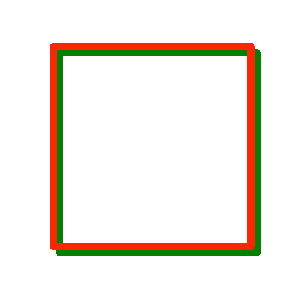
\includegraphics[width=0.5\linewidth]{graphics/iou/iou_examples/3.pdf}
        \caption*{Sehr gut} 
        \vspace{2ex}
    \end{subfigure}
    
    \caption*{Quelle: \textcite{IoU}}
\end{figure}

\subsubsection{Average Precision}
\label{chap:ap}

Average Precision, kurz AP, ist eine Metrik, welche oft bei der Bewertung von Modellen zur Objekterkennung zur Anwendung kommt. Als Average Precision wird der Durchschnitt aller Genauigkeiten bei jeder Sensitivität verstanden. Um dies genauer zur erläutern wird im Folgenden ein Beispiel zur Berechnung aufgeführt~\autocite{AP}.

Wird ein Modell zur Erkennung von fünf Katzen auf zehn Bildern angewendet, so sind insgesamt fünf True Positive Beispiele vorhanden. Die Tabelle \ref{tab:ap-example} zeigt mögliche Ergebnisse des Modells. Die Ergebnisse sind sortiert nach der Konfidenz des Modells, richtig zu liegen. Pro Vorhersage wird nun die Genauigkeit sowie die Sensitivität berechnet. Dabei steigt die Sensitivität bei jeder korrekten Vorhersage. Die Genauigkeit steigt bei jeder korrekten Vorhersage und sinkt bei jeder falschen~\autocite{AP}.

\begin{table}[h!]
    \captionsetup{width=.9\linewidth}
    \caption{Beispiel der Berechnung der Genauigkeit und Sensitivität als Grundlage zur Berechnung der Average Precision}
    \label{tab:ap-example}
    \centering
    \begin{tabular}{|l|l|l|l|} 
    \hline
    Rang & Korrekte Vorhersage & Genauigkeit & Sensitivität  \\ 
    \hline
    1    & Ja                  & 1.0         & 0.2           \\ 
    \hline
    2    & Ja                  & 1.0         & 0.4           \\ 
    \hline
    3    & Nein                & 0.67        & 0.4           \\ 
    \hline
    4    & Nein                & 0.5         & 0.4           \\ 
    \hline
    5    & Nein                & 0.4         & 0.4           \\ 
    \hline
    6    & Ja                  & 0.5         & 0.6           \\ 
    \hline
    7    & Ja                  & 0.57        & 0.8           \\ 
    \hline
    8    & Nein                & 0.5         & 0.8           \\ 
    \hline
    9    & Nein                & 0.44        & 0.8           \\ 
    \hline
    10   & Ja                  & 0.5         & 1.0           \\
    \hline
    \end{tabular}
    \caption*{Quelle: \textcite{AP}}
\end{table}

Die Abbildung \ref{fig:ap-pr} zeigt die sogenannte PR-Curve (Precision-Recall-Curve), welche die Genauigkeit bei jeder Sensitivität darstellt, für das genannte Beispiel. Auf der Abbildung ist die Zickzack Linie durch die steigende und sinkende Genauigkeit zu erkennen~\autocite{AP}.

\begin{figure}[H]
    \captionsetup{width=.9\linewidth}
    \caption{Beispiel einer PR-Curve, die die Genauigkeit bei der Sensitivität darstellt.}
    \label{fig:ap-pr}
    \centering
    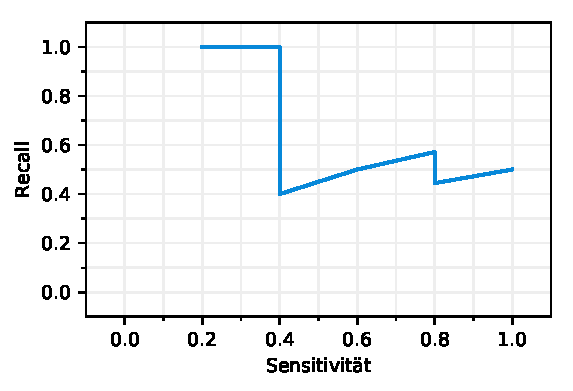
\includegraphics[scale=1]{graphics/matplot/ap__pr.pdf}\\
    \caption*{Quelle: \textcite{AP}}
\end{figure}

Wie erwähnt, wird als Average Precision der Durchschnitt aller Genauigkeiten bei jeder Sensitivität verstanden. Die Average Precision wird generell als die Fläche unter der PR-Curve definiert~\autocite{AP}:

$$AP = \int_{0}^{1}p(r)dr$$

Da sowohl die Genauigkeit als auch die Sensitivität zwischen 0 und 1 liegt, fällt auch die Average Precision zwischen 0 und 1~\autocite{AP}.

Um die Berechnung der Average Precision zu vereinfachen, wird die Zickzack Linie oftmals geglättet. Dabei wird zu jeder Sensitivität jeweils die maximale Genauigkeit aller grösseren Sensitivitäten gewählt~\autocite{AP}. Die grüne Linie in Abbildung \ref{fig:pr-smoothed} veranschaulicht diese Glättung.

\begin{figure}[H]
    \captionsetup{width=.9\linewidth}
    \caption{Beispiel zur Glättung einer PR-Curve}
    \label{fig:pr-smoothed}
    \centering
    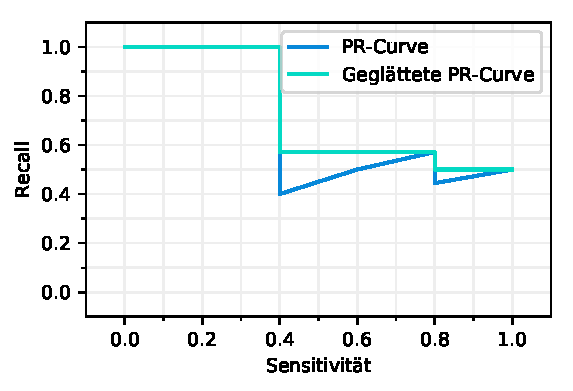
\includegraphics[scale=1]{graphics/matplot/ap__pr-smoothed.pdf}\\
    \caption*{Quelle: \textcite{AP}}
\end{figure}

Neben dieser Glättung kommt in gewissen Fällen auch eine Interpolation zur Anwendung. Bis 2008 verwendete das PASCAL VOC Dataset zur Berechnung der Average Precision eine Interpolation mit elf Punkten. Das bedeutet, dass die Genauigkeit bei allen Sensitivitäts-Werten mit dem Faktor 0.1 berechnet wird. Beim COCO\footnote{Das COCO (Common Objects in Context) Dataset ist ein sehr grosses Dataset, welches für diverse Wettbewerbe im Bereich der Objekterkennung verwendet wird.} Dataset wird eine Interpolation von 101 Punkten verwendet. Im neueren PASCAL VOC Dataset\footnote{Die PASCAL Visual Object Classes Datasets sind ein annotierte Datensätze zur Objekterkennung auf Bildern, welche von 2005 bis 2012 für die PASCAL VOC Challenge ausgegeben wurden.} wird auf eine Interpolation verzichtet und die Average Precision wird als die Fläche unter der geglätteten PR-Curve berechnet. Je nach Art der Berechnung kann es zu unterschiedlichen Resultaten kommen, wie dies Abbildung \ref{fig:pr-interpolated} zeigt. Durch die Interpolation können Ungenauigkeiten entstehen, wenn die Abnahme der Genauigkeit nicht genau auf einen der zur Berechnung verwendeten Punkte fällt. Werden Modelle miteinander verglichen, ist es also wichtig zu wissen, welche Methode zur Berechnung verwendet wurde~\autocite{AP}.

\begin{figure}[H]
    \captionsetup{width=.9\linewidth}
    \caption{Interpolation einer geglätteten PR-Curve.}
    \label{fig:pr-interpolated}
    \centering
    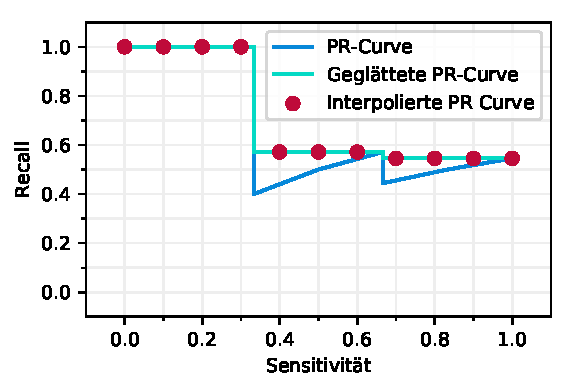
\includegraphics[scale=1]{graphics/matplot/ap__pr-interpolated.pdf}\\
    \caption*{Quelle: \textcite{AP}}
\end{figure}

\subsubsection{Mean Average Precision}
\label{chap:map}

Als Mean Average Precision (kurz mAP) wird der Durchschnitt über mehrere Average Precisions bezeichnet. Welche Average Precisions dabei gemeint sind, ist von Anwendung zu Anwendung unterschiedlich. In gewissen Fällen wird einfach nur von der Average Precision gesprochen, obwohl eigentlich ein Durchschnitt über mehrere Average Precisions gemeint ist. Es wird davon ausgegangen, dass dies im Kontext klar ist. Im Folgenden werden drei Varianten zur Bildung der Mean Average Precision erläutert~\autocite{AP}.

Im COCO Dataset wird der Durchschnitt der Average Precisions für unterschiedliche Schwellenwerte für das Intersection over Union Verfahren als Mean Average Precision bezeichnet. Konkret werden alle Average Precisions für die IoU Schwellenwerte in Schritten von 0.05 zwischen 0.5 und 0.95 gemittelt. Dies wird dabei als $mAP[0.5:0.05:0.95]$ oder kürzer $mAP[0.5:0.95]$ bezeichnet. Durch dieses Verfahren werden Modelle mit genaueren Vorhersagen, sprich grösserem IoU Wert, besser bewertet~\autocite{AP}.

In anderen Fällen wird Mean Average Precision als der Durchschnitt der Average Precisions über alle zu identifizierenden Klassen berechnet. Sollen in einer Aufgabe Hunde und Katzen auf Bildern erkannt werden, so kann für beide Klassen eine Average Precision ermittelt werden. Ein Modell könnte eine Average Precision für Hunde von 0.9 und eine für Katzen von 0.3 aufweisen. Um dieses Modell nun mit einem anderen Modell zu vergleichen, wird die Mean Average Precision über alle Klassen berechnet~\autocite{AP}:

$$mAP = \frac{\sum_{i=0}^{n}AP_{i}}{n} = \frac{AP_{Hund}+AP_{Katze}}{2} = 0.6$$

Die beiden Methoden werden oft kombiniert, um somit die Mean Average Precision über mehrere Intersection over Union Schwellenwerte und über mehrere Klassen zu berechnen. Dies ermöglicht, verschiedene Modelle mit nur einer Zahl zu vergleichen~\autocite{AP}.

\subsection{Fehleranalyse}
\label{chap:error-analysis}

Als Fehleranalyse wird die Analyse der falschen Vorhersagen eines Modells bezeichnet. Im Falle eines Klassifizierungsmodells werden die falsch klassifizierten Datensätze betrachtet und auf die Ursache der falschen Klassifizierung untersucht. Das Ziel dabei ist es, Optimierungspotential zu finden, anhand welchem das bestehende Modell verbessert werden kann~\autocite{MLYearning}.

Wird beispielsweise ein Modell zur Klassifizierung von Bildern in die Klassen Hund und Katze mit einer Treffergenauigkeit von 90\% untersucht, so könnte eine Erkenntnis sein, dass nur 5\% aller falsch Klassifizierten Bilder der Klasse Hund angehören. Es würde nun wenig Sinn machen, das Modell zur besseren Erkennung von Hunden zu optimieren. Es könnte dadurch nur 5\% des Fehlers reduziert, sprich 0.5\% an Treffergenauigkeit gewonnen werden. Würden 50\% der falsch Klassifizierten Bilder der Klasse Hund angehören, würde eine solche Optimierung Sinn machen, denn die Reduktion der Fehler um 50\% würde eine Steigerung der Treffergenauigkeit von 5\% (50\% der Fehlerquote von 10\%) ermöglichen~\autocite{MLYearning}.

Die Fehleranalyse hilft die Ursachen einer falschen Klassifizierung zu finden. Sie kann somit Auskunft darüber geben, in welche Richtung das untersuchte Modell optimiert respektive weiterentwickelt werden soll~\autocite{MLYearning}.

%- Betrachtung der Falsch Klassifizierten Daten
%- Ziel: Optimierungspotential finden
%- Beispiel 5\% der falsch Klassifizierten Bilder sind Hunde. Egal wie startk für Hunde optimiert wird, es wird maximal 5\% des Fehlers optimiert
%- Fehleranalyse zeigt, in welche Richtung weiter vorgegangen werden soll
%- Fehleranalyse hilft die Ursachen der Falschklassifizierung zu finden
%- Kann helfen, unbekannte Gebiete durch ein iteratives vorgehen zu explorieren

\subsubsection{Design eines KI Systems}

Die vorherigen Kapitel haben einen Einblick in einige der Grundbausteine von Machine Learning Modellen gegeben. Eine grosse Herausforderung ist nun, diese so anzuwenden, dass eine Problemstellung möglichst optimal gelöst werden kann. Dieses Kapitel gibt einen Überblick, wie an eine Problemstellung herangegangen werden soll, um ein Machine Learning Modell zu entwickeln.

% - https://towardsdatascience.com/machine-learning-general-process-8f1b510bd8af
Der erste und einer der wichtigsten Schritte ist, die \textbf{Problemstellung zu beschreiben}. Dabei gilt es zu klären, was das genau Ziel ist respektive was vorhergesagt werden soll. Das heisst, es muss geklärt werden, wie genau die Ausgabe des Modells aussehen soll. Es ist ausserdem zu klären, welche Daten als Eingabewerte notwendig und ob diese verfügbar sind. Weiter gilt es zu definieren, anhand welcher Metrik das Modell gemessen wird~\autocite{DesignML}.

Der nächste Schritt ist die \textbf{Beschaffung der identifizierten Daten}. In gewissen Fällen ist dieser Schritt einfach, in anderen aufwendig. Für gewisse Problemstellungen sind bereits strukturierte Daten vorhanden. Bei anderen müssen diese mit aufwendigen Techniken wie Web-Scraping, dem automatisierten extrahieren von Informationen aus Webseiten, beschafft werden~\autocite{DesignML}.

Im dritten Schritt muss eine \textbf{Zielmetrik} bestimmt werden. Das Kapitel \ref{chap:metrices} zeigt einige der bekanntesten Metriken auf. Die Wahl der Metrik ist wichtig, damit das Ziel bekannt und das Modell auf die Erreichung dieses optimiert werden kann~\autocite{DesignML}.

Nachdem das Ziel bekannt ist, müssen die \textbf{Eingabedaten aufbereitet} werden. Dabei muss ein Weg gefunden werden, mit potentiell fehlenden oder unvollständigen Daten umzugehen. Alle Daten müssen in eine Form gebracht werden, welche das Modell verstehen kann. So müssen beispielsweise ordinale und nominale Daten in Ganzzahlen umgewandelt respektive codiert werden. Da die meisten Modelle mit gleich skalierten Daten am besten umgehen können, werden die Daten auf die Skala $[0:1]$ gebracht~\autocite{DesignML}.

Lassen die Problemstellung und die Eingabedaten es zu, so ist es Ratsam nun eine \textbf{einfache Vorhersage}\todo{Anderes Wort}, beispielsweise basierenden auf k-Nearest-Neighbour\footnote{k-Nearest-Neighbour ist ein Algorithmus zur Klassifizierung eines Datensatzes aufgrund seiner k-nächsten Nachbarn, sprich k-ähnlichsten Datensätzen.} oder Naive Bayes\footnote{Naive Bayes ist ein Algorithmus zur Klassifizierung, welcher Datensätze aufgrund einer Kostenfunktion klassifiziert. Ein Datensatz wird jener Klasse zugewiesen, bei welcher die wenigsten Kosten entstehen.}, zu erstellen. Eine solche Vorhersage ermöglicht die Eingabedaten auf ihre Eignung zur Vorhersage des gesuchten Resultats zu prüfen. Weiter gibt diese Vorhersage eine Baseline, an welcher sich während der Erarbeitung des Machine Learning Modells gehalten werden kann.~\autocite{DesignMLSecondaryCite}

Nachdem alle Rahmenbedingungen geschaffen sind, geht es nun an die \textbf{Entwicklung des Modells}. Dabei ist Cross Validation, der Vergleich von bestehenden Modellen, und das anschliessende Optimieren des besten Kandidaten, ein oft angewendetes Vorgehen. Beim Cross Validation werden verschiedene Modelle auf den Eingabedaten angewendet und anhand der Zielmetrik bewertet. Das Modell mit dem besten Resultat wird anschliessend optimiert. Diese Optimierung ist die Anpassung der sogenannten Hyperparametern. Die Hyperparameter bezeichnen jene Parameter eines Machine Learning Modells, welche nicht während dem Training gelernt, sondern von aussen in das Modell hereingegeben werden. Die Hyperparameter können als Konfiguration eines Modells verstanden werden~\autocite{DesignML}.

\todo[inline, color=red]{Rest dieses Kapitels zu Neural Network Design schreiben. Gute Quellen suchen

- ftp://ftp.sas.com/pub/neural/FAQ3.html\#A\_hl

Um eine Problemstellung mit einem Neuronalen Netzwerk zu lösen, muss erst ein solches entworfen werden. Auch hier ist der Cross Validation Ansatz wohl der geeignetste, um möglichst schnell gute Resultate zu erzielen. Für viele Problemstellungen können Analogien gefunden werden, zu welchen bereits Modelle bestehen. Es gibt diverse Wettbewerbe, bei welchen Modelle, beispielsweise zur Objekterkennung auf Bildern, verglichen werden. Auch gibt es unzählige frei verfügbare Forschungsarbeiten und Open Source Modelle, welche Lösung zu einer breiten Variation von Problemstellungen präsentieren.

Wird ein Modell selbst entworfen oder angepasst, so stellt sich oft die Frage, wie viele Hidden Layer ein solches Modell haben sollte und wie viele Neuronen diese beinhalten sollen. Für diese Frage gibt es keine klare Antwort. 


Beim Entwurf eines solches Netzwerks stellt sich die Frage, was für Schichten und wie viele davon ein Netzwerk haben soll. Es gibt dafür in vielen Fällen keine klaren Regeln und es muss oft etwas experimentiert werden. Einige Faustregeln können dabei helfen, mit geringem Aufwand ein geeignetes Modell zu finden.
}

\subsection{Künstliche Intelligenz in produktiver Umgebung}

\todo[inline, color=red]{
- KI/ML beginnt oft mit Experimenten

- KI Software in stetigem Wandel

- Verschiedene ML Architekturen: https://towardsdatascience.com/five-not-well-known-machine-learning-architectures-that-will-help-you-move-from-pilot-to-production-a051eaae69ef

- Uber hat mit Michelangelo eine extrem fortgeschrittene Pipeline, evtl. helfen Erkenntnise daraus

-- https://eng.uber.com/michelangelo/

-- Learning in production wird gemäss diesem Post auch bei Uber nicht gemacht. Lernen passiert aktuell immer offline

-- Lernen in Produktion muss extrem stark überwacht werden, da sonst das Modell Amok laufen könnte

}

